% -------------------------------------------------------------------------------------------------
%      MDSG Latex Framework
%      ============================================================================================
%      File:                  main.tex
%      Author(s):             Michael Duerr
%      Version:               1
%      Creation Date:         30. Mai 2010
%      Creation Date:         30. Mai 2010
%
%      Notes:                 - This represents the document root of this template
%                             - Binding correction is 12mm. In case you change this value, you
%                               may also need to adapt the value of \bcorlength in mdsg.sty
%                             - Switch `babel' package options `english' and `ngerman' in case
%                               your thesis is in English
%                             - if you prefer to use utf8 encoding, uncomment the corresponding
%                               line `\usepackage[utf8]{inputenc}' and comment the line
%                               `\usepackage[latin1]{inputenc}'. To compile this example you also
%                               need to include the corresponding introduction example file i.e.
%                               `introduction-UTF8.tex' or `introduction-ISO8859-1.tex'
% -------------------------------------------------------------------------------------------------
%
\documentclass[bibliography=totoc,listof=totoc,index=totoc,twoside=true,BCOR=12mm,DIV=12]{scrbook}
%\KOMAoptions{draft=true}                         % uncomment if you want to visualise overful hbox
%\KOMAoptions{chapterprefix=true}                 % uncomment if you like "Chapter" in front of
                                                  % chapter number
%\KOMAoptions{appendixprefix=true}                % uncomment if you like "Appendix" in front of
                                                  % appendix number
%\KOMAoptions{...}                                % feel free to add additional KOMA options
%
% =================================================================================================
% set encoding
% -------------------------------------------------------------------------------------------------
%
\usepackage[utf8]{inputenc}                       % uncomment if you prefer utf8 encoding
%\usepackage[latin1]{inputenc}                    % uncomment if you prefer latin1 encoding
%
% =================================================================================================
% load mdsg style
% -------------------------------------------------------------------------------------------------
%
%\usepackage[diplom]{mdsg}                        % uncomment the corresponding option
%\usepackage[fopra]{mdsg}
%\usepackage[bachelor]{mdsg}
\usepackage[master]{mdsg}
%
% =================================================================================================
% initialize macros
% -------------------------------------------------------------------------------------------------
%
\lmutitle{Titel der Arbeit}                       % title: you can force a new line by
%\lmutitle{Titel \\ der \\ Arbeit}                % inserting `\\'. However, this will cause
                                                  % a hyperref warning!
\lmustudentone{Judith Greif}                    	 % first author's name
%\lmustudenttwo{Max2 Mustermann2}                 % second author's name
%\lmustudentthree{Max3 Mustermann3}               % third author's name
%\lmustudentfour{Max4 Mustermann4}                % fourth author's name

\lmuprofone{Prof. Dr. Claudia Linnhoff-Popien}    % first supervisor's name
%\lmuproftwo{Prof. Dr. Max Mustermann}             % second supervisor's name
                                                  % (uncomment if not needed)
%\lmuprofthree{Prof. Dr. Max2 Mustermann2}         % third supervisor's name
                                                  % (uncomment if not needed)
\lmuadvisorone{Mirco Schönfeld}                    % first advisor's name
\lmuadvisortwo{Dr. Martin Werner}                    % second advisor's name
                                                  % (uncomment if not needed)
%\lmuadvisorthree{Betreuer Name3}                  % third advisor's name
                                                  % (uncomment if not needed)
\lmudraftdate{\today}                             % only for versioning during work!
                                                  % (uncomment for final version!)
\lmudeadline{1. Januar 2099}                      % deadline (day of submission)
%
% =================================================================================================
% package selection (add additional packages if needed)
% -------------------------------------------------------------------------------------------------
%
%\usepackage{layout}                              % see documentation of this package
\usepackage{cmap}                                 % to produce searchable PDF
\usepackage[T1]{fontenc}                          % split german words with umlaut
\usepackage{lmodern}
\usepackage[english,ngerman]{babel}               % for german toc, ...
\usepackage{bibgerm}                              % for german bibliography index
\usepackage{tabularx}                             % more flexible table environment
\usepackage{booktabs}                             % high quality tables
\usepackage{rotating}                             % for generation of landscape tables
\usepackage{multirow}                             % for multirow cells inside tables
\usepackage{amssymb,amsmath}                      % powerful math package
\usepackage{hyperref}                             % for hyperlinks
\lmuhypersetup                                    % write some pdf properties
\usepackage{flafter}                              % force floats to appear after their reference
\usepackage{subfig}                               % to allow for side by side graphics (subfloats)
\usepackage{pdflscape}                            % enable rotation of landscape pages
\usepackage{hyphenat}                             % proper hyphenation for bla_bla to bla_-bla
\usepackage[all]{hypcap}                          % correct captions
\usepackage{url}                                  % nicer url style
\usepackage{enumitem}                             % for tight lists
\usepackage{textcomp}
%\usepackage{...}                                 % add additional packages here

\setcounter{tocdepth}{3}                          % sectioning depth in toc
\setcounter{secnumdepth}{3}                       % sectioning depth in text

\graphicspath{{./pictures/}}                      % put all graphics here
% -------------------------------------------------------------------------------------------------
%      MDSG Latex Framework
%      ============================================================================================
%      File:                  hyphenation.tex
%      Author(s):             Michael Duerr
%      Version:               1
%      Creation Date:         30. Mai 2010
%      Creation Date:         30. Mai 2010
%
%      Notes:                 - Instruction \hypenation cannot handle special characters like umlaute
%                               as well as  "a and \"a. Split such words in your text.
%
% -------------------------------------------------------------------------------------------------
%
\hyphenation{Ba-che-lor-ar-}
%\hyphenation{...}                           % further hyphenation examples
                               % this file holds words latex cannot split
%
% =================================================================================================
% start of document
% -------------------------------------------------------------------------------------------------
%
\begin{document}
    \setlist{noitemsep}                           % for tight lists
    \lmufront                                     % title pages
    \newpage
    \cleardoublepage
    \lmuaffirmation                               % affirmation (work is my own work)
    \newpage
    \cleardoubleemptypage
    \thispagestyle{empty}
    % -------------------------------------------------------------------------------------------------
%      MDSG Latex Framework
%      ============================================================================================
%      File:                  abstract.tex
%      Author(s):             Michael Duerr
%      Version:               1
%      Creation Date:         30. Mai 2010
%      Creation Date:         30. Mai 2010
%
%      Notes:                 - Place your abstract here
% -------------------------------------------------------------------------------------------------
%
\vspace*{2cm}

\begin{center}
    \textbf{Abstract}
\end{center}

\vspace*{1cm}

\noindent Ubiquitous computing und die Zunahme mobiler Endgeräte haben zu neuen Kommunikationsmustern im Internet geführt: Weg von adressbasiertem Routing und Ende-zu-Ende-Kommunikation hin zu \textit{Information-centric Networking}. Kontextzentrische soziale Netze sind ein Ansatz, dem Rechnung zu tragen. Kommunikation basiert darin nicht auf Online-Freundschaft, sondern allein auf Kontext-Ähnlichkeit. Das kontextzentrische soziale Netz AMBIENCE verwendet Bloom-Filter, um Nachrichten zu kodieren, speichern und anzufragen. Diese müssen so an einem Host organisiert werden, dass die \textit{k} nächsten Nachbarn zu einem Anfragefilter möglichst schnell und effizient gefunden werden. Die vorliegende Arbeit optimiert das mengentheoretische Problem der \textit{k}-nächsten-Nachbarn-Suche für dieses Szenario. Dazu wurde eine Indexstruktur für Bloom-Filter basierend auf einem B$^+$-Baum entwickelt. Die Bloom-Filter werden darin nach ihren Teil- und Obermengenbeziehungen organisiert, der \textit{BloomFilterTree}. Bei der \textit{k}-nächsten-Nachbarn-Suche wird nur der beste Pfad im Baum verfolgt und Teilbäume möglichst früh abgeschnitten. Kriterien für die Evaluation waren Ergebnisqualität, CPU-Zeit, Zeitkomplexität, Speicherbedarf und Aufbaukosten. Im verwendeten Versuchsaufbau ließen sich Zeitkomplexität und CPU-Zeit der \textit{k}-nächste-Nachbarn-Suche mit dem BloomFilterTree um bis zu 68\% bzw. 87\% reduzieren.                        % abstract
    \thispagestyle{empty}
    \frontmatter                                  % start roman numbering
    \tableofcontents                              % toc
    \mainmatter                                   % start alpha numbering
%
% =================================================================================================
% place your document text here (take care of encoding)
% -------------------------------------------------------------------------------------------------
%
    \chapter{Einleitung}\label{sec:Introduction}
%\section{Erstes Unterkapitel}
%\subsection{Quellenangaben}\label{subsec:sources}
Wir zitieren hier die Quellen \cite{Agarwal2006}, \cite{Ahlgren2012}, \cite{Bayardo2007}, \cite{Broder2004}, \cite{Byers2002}, \cite{Duerr2010}, \cite{Hellerstein1994}, \cite{Lehman1986}, \cite{Mitzenmacher2002}, \cite{Nafe2005}, \cite{Qiao2014}, \cite{Ruppel2014}, \cite{Sakuma2011}, \cite{Sarwat2012}, \cite{Schnell2013}, \cite{Schoenfeld2014}, \cite{Shiraki2009}, \cite{Werner2015}, \cite{Yang2002}, \cite{Zhang2012}, \cite{Zhu2004}, die in der Datei\\
\verb|bibliography.bib|
stehen.
%\subsection{Referenz auf anderen Text}
%Es ist auch möglich auf andere Stellen im Text z.B. Kapitel \ref{subsec:sources} zu verweisen.
%\subsection{Tabellen}
%Es gibt schöne Möglichkeiten Tabellen einzubinden wie z.B. Tabelle \ref{tab:CommonParameterSettings}.
%\begin{center}
%\begin{table}[htbp]
%{\small
%\begin{center}
%\begin{tabular}[center]{lrlc}
%\toprule
%Parameter & Value & (Unit) & Available for Chord \\
%\midrule
%Query timeout & 10 & seconds & $\surd$ \\
%Republish timeout & 300 & seconds & $\surd$ \\ % explain this value...
%Stabilize timeout & 5 & seconds & $\surd$ \\
%Fix fingers timeout & 30 & seconds & $\surd$ \\
%Message timeout & 1 & second & $\surd$ \\
%Connect timeout & 10 & seconds & $\surd$ \\
%Ping superpeer timeout & 5 & seconds & $\times$ \\
%Cost-Optimality estimation timeout & 20 & seconds & $\times$ \\
%Significance for change in number of superpeers & 10 & percent & $\times$ \\
%Significance for change in estimations  & 10 & percent & $\times$ \\
%Number of permanent superpeers & 32 & nodes & $\times$ \\
%Mean number of peers & 1000 & nodes & $\surd$ \\
%Mean number of lookups per hour & 60 & queries & $\surd$ \\
%Mean number of shared InfoProfiles per node & 20 & & $\surd$ \\
%Identifier space & 16 & bits & $\surd$ \\
%Direct insertion acknowledgment & true & bool & $\times$ \\
%Direct query responses & true & bool & $\times$ \\
%Force query resolution & true & bool & $\surd$  \\
%\bottomrule
%\end{tabular}
%\end{center}
%} % end of tiny
%\caption[Simulation parameter settings]{Common simulation parameter settings.\label{tab:CommonParameterSettings}}
%\end{table}
%\end{center}
%
%\subsection{Bilder}
%Man kann sehr einfach Bilder einbinden so wie z.B. in Abbildung \ref{fig:pic0}.
%\begin{figure}[hpbt]
%  \centering
%  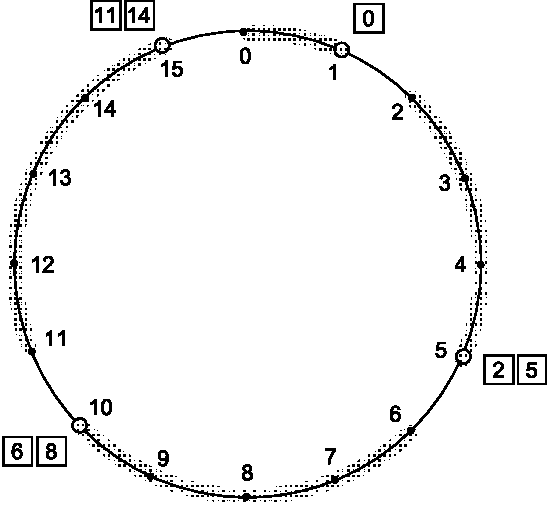
\includegraphics[width=0.4\textwidth]{pictures/pic0}\\
%  \caption[Example of a $4$-bit Chord identifier circle]{Example of a $4$-bit Chord identifier circle.
%  The responsibility ranges for each peer are accentuated in light gray}\label{fig:pic0}
%\end{figure}
%Es lassen sich auch mehrere Bilder nebeneinander platzieren wie z.B. in Abbildung
%\ref{fig:multipic} zu sehen ist.
%\begin{figure}[hpbt]
% \centering
%  %%----start of first subfigure----
%  \subfloat[FIFO size limited to 20 entries]{
%   \label{fig:multipic:a} %% label for first subfigure
%   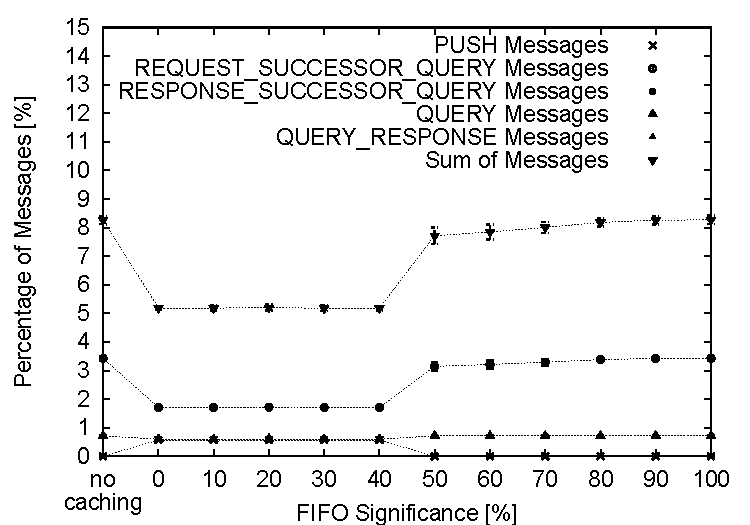
\includegraphics[width=0.48\linewidth]{pic1}}
%  \hspace{0.01\textwidth}
%  %%----start of second subfigure----
%  \subfloat[FIFO size limited to 30 entries]{
%   \label{fig:multipic:b} %% label for second subfigure
%   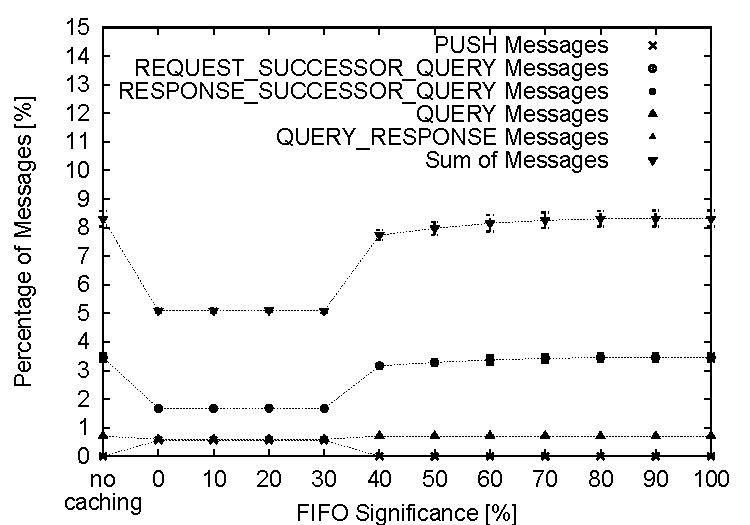
\includegraphics[width=0.48\linewidth]{pic2}}\\[0pt] % horizontal break
%  %%----start of third subfigure----
%  \subfloat[FIFO size limited to 40 entries]{
%   \label{fig:multipic:c} %% label for third subfigure
%   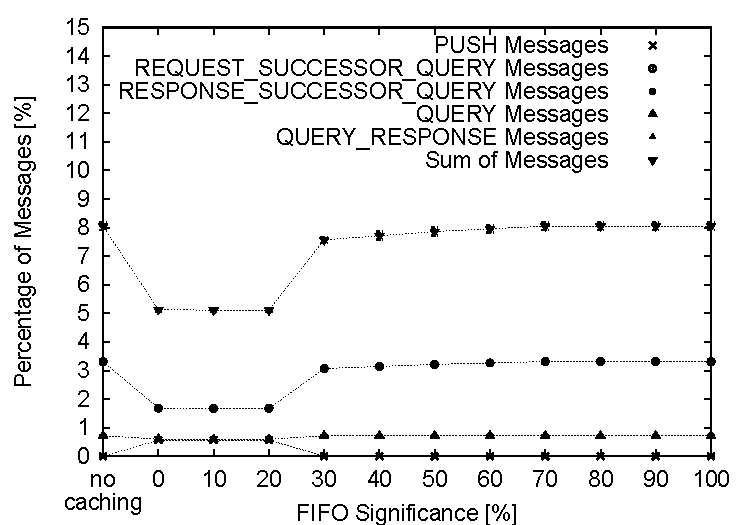
\includegraphics[width=0.48\linewidth]{pic3}}
%  \hspace{0.01\textwidth}
%  %%----start of fourth subfigure----
%  \subfloat[FIFO size limited to 50 entries]{
%   \label{fig:multipic:d} %% label for fourth subfigure
%   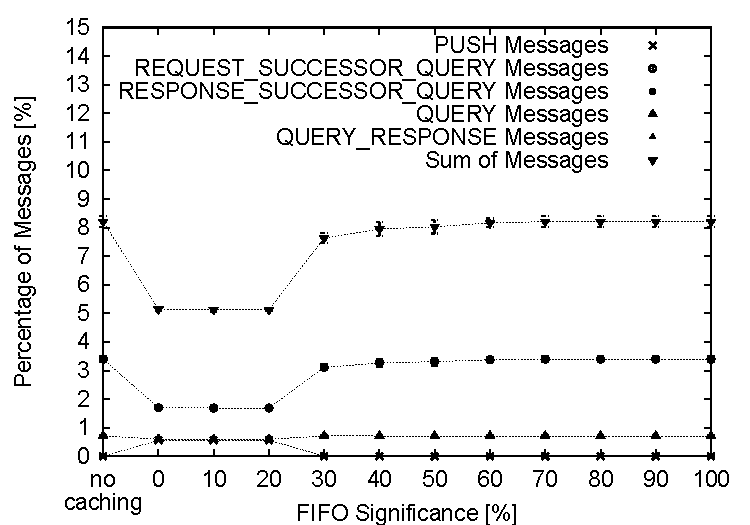
\includegraphics[width=0.48\linewidth]{pic4}}
% \caption[Observed message fractions and 95\% confidence intervals for Chord]{Observed message fractions and 95\% confidence intervals for Chord without the influence of churn. The FIFO capacity varies from 20 (\ref{fig:multipic:a}) -- 50 (\ref{fig:multipic:d}) entries (decadic steps).}
% \label{fig:multipic} %% label for entire figure
%\end{figure}
%
%\subsection{Programm Code}
%Eine elegante Möglichkeit, Programmtext einzubinden, lässt sich mit dem listings-Paket erreichen.
%Das \verb|HelloWorld| Programm aus Listing \ref{lst:hw} hat in Zeile \ref{line:hw3} übrigens einen Programmierfehler.
%\begin{lstlisting}[float=htp,caption=Hello World,label=lst:hw,language=Java, numbers=left, numberstyle=\tiny, stepnumber=2, numbersep=8pt, escapeinside={//@}{@//},backgroundcolor=\color{yellow},xleftmargin=3ex,xrightmargin=1ex]
%public class HelloWorld {
%    public static void main(String[] args) {
%        Syste.out.println("Hello, World"); //@\label{line:hw3}@//
%    }
%}
%\end{lstlisting}
    \chapter{Background}\label{ch:background}
\section{Bloom Filters}\label{sec:bloom}
\subsection{Classic Bloom Filter}\label{subsec:classic_bloom}
\cite{Bloom1970}
\subsection{Bloom Filter Operations and Variants}\label{subsec:bloom_ops}
\textit{Attenuated Bloom Filter:} \cite{Sakuma2011}: 316 and 318\\
\textit{Counting Bloom Filter:} \cite{Fan2000}\\
\textit{Compressed Bloom Filter:} \cite{Mitzenmacher2002}
\section{Mathematic Principles}\label{sec:math}
\section{Index Structures in Database Systems}\label{sec:index_structures}
To support query processing and operations in an efficient manner, the internal layer of a database system uses specific data strucures and memory methods. These are called \textit{index structures}. They organize the data to support the required operations using its \textit{indices}.

An \textit{index} (also called \textit{directory}) of a file holds information about its structure. A \textit{file} in this context refers to an entire data structure, i.e. an array, a search tree etc.. One can differentiate between three classes of index structures depending on the manner of organization: 
\begin{enumerate}
	\item \textbf{\textit{Data-organizing index structures}} are used to organize the actual amount of data. They mostly rely on \textit{search trees}. 
	\item \textbf{\textit{Space-organizing index structures}} are used to organize the space that holds the data. They make use of \textit{dynamic hashing}. 
	\item \textbf{\textit{Hybrid index structures}} are a combination of both classes. They are based on \textit{hash trees}.   
\end{enumerate}
There are several requirements for an index structure in order to meet its purpose. 
\begin{itemize}
	\item \textit{Efficient search:} A data query on the index structure should return an answer in optimal time, i.e. the query should be directed to the page or pages that contain the queried data using as little steps as possible.
	\item \textit{Dynamic insertion, deletion and modification of data sets:} The amount of data to be organized changes over time, leading to alterations in the index structure as well. Any implementation requiring a complete reorganization of the index structure on insertion, deletion or modification of data sets is clearly unacceptable. Any of these operations may therefore only lead to local changes. 
	\item \textit{Local preservation of order:} If there are some data sets the keys of which are successors within the applied order relation (i.e. the less-or-equal relation on non-negative integers), this order should be preserved within the index structure. This holds for search trees but it does not hold for linear hashing. It is clearly of great importance regarding the application scenario in question.
	\item \textit{Efficient use of space:} This requirement is of great importance for real-world applications. So far the reference implementation \textit{AMBIENCE} has served as a proof of concept. Accordingly the number of messages, i.e. the amount of data to be queried, has been relatively small compared to a real-world scenario. Therefore the memory requirements of any index structure within the current scenario that represents the actual amount of data is unlikely to require vast amounts of memory. However, keeping in mind future application scenarios for \textit{AMBIENCE}, efficient use of space cannot be entirely discarded. 
\end{itemize}
Further requirements include \textit{feasability} and \textit{implementation cost}. Any index structure aiming at a real-world implementation such as \textit{AMBIENCE} naturally has to be feasable, so this requirement will be overlooked in the following. As this work clearly has a scholarly background, not an industrial one, the implementation cost will be disregarded as well.\\ 
\cite{Ottmann2012}
\subsection{B-Tree}	
\cite{Knuth1998}	
\subsection{R-Tree}
% "Ein R-Baum (englisch R-tree) ist eine in Datenbanksystemen verwendete mehrdimensionale (räumliche) dynamische Indexstruktur. Ähnlich wie bei einem B-Baum handelt es sich hier um eine balancierte Indexstruktur" (vgl. https://de.wikipedia.org/wiki/R-Baum)
\subsection{R*-Tree}
% "Eine beliebte R-Baum-Variation ist der R*-Baum von Norbert Beckmann, Hans-Peter Kriegel, Ralf Schneider und Bernhard Seeger. Diese Variante versucht, durch eine weiterentwickelte Split-Strategie das Überlappen von Rechtecksregionen zu minimieren. Dadurch brauchen bei einer Suchanfrage meistens weniger Teilbäume durchsucht zu werden, und die Anfragen an den Baum werden dadurch effizienter. Zusätzlich können beim Überlauf einer Seite auch Elemente neu in den Baum eingefügt werden (re-insert), was eine Aufteilung (engl. "split") (und die damit unter Umständen steigende Höhe des Baumes) vermeiden kann. Dadurch wird ein höherer Füllgrad erreicht und dadurch ebenfalls eine verbesserte Effizienz. Der resultierende Baum ist aber stets auch ein R-Baum, die Anfragestrategie ist unverändert" (vgl. https://de.wikipedia.org/wiki/R-Baum\#R.2A-Baum)
\subsection{Heap}
% "Ein Heap (englisch wörtlich: Haufen oder Halde) in der Informatik ist eine zumeist auf Bäumen basierende abstrakte Datenstruktur. In einem Heap können Objekte oder Elemente abgelegt und aus diesem wieder entnommen werden. Sie dienen damit der Speicherung von Mengen. Den Elementen ist dabei ein Schlüssel zugeordnet, der die Priorität der Elemente festlegt. Häufig werden auch die Elemente selbst als Schlüssel verwendet. Über die Menge der Schlüssel muss daher eine totale Ordnung festgelegt sein, über welche die Reihenfolge der eingefügten Elemente festgelegt wird. Beispielsweise könnte die Menge der ganzen Zahlen zusammen mit der Kleinerrelation (<) als Schlüsselmenge fungieren. Der Begriff Heap wird häufig als bedeutungsgleich zu einem partiell geordneten Baum verstanden [...]. Gelegentlich versteht man einschränkend nur eine besondere Implementierungsform eines partiell geordneten Baums, nämlich die Einbettung in ein Array, als Heap" (vgl. https://de.wikipedia.org/wiki/Heap\_(Datenstruktur))
\section{AMBIENCE}\label{sec:ambience}
\cite{Werner2015}. 
    \chapter{Implementation}\label{ch:implementation}


    \chapter{Evaluation}\label{ch:evaluation}
Das folgende Kapitel dient dem Vergleich zwischen der entwickelten Datenstruktur und der bisherigen Organisation der Bloom-Filter in AMBIENCE. Abschnitt \ref{sec:datensatz} beschreibt zunächst den für die Evaluation verwendeten Datensatz. Dieser stammt nicht aus AMBIENCE, sondern die Bloom-Filter wurden wie in Abschnitt \ref{sec:umsetzung} beschrieben selbst implementiert. Der Versuchsaufbau, d.h. welche Aspekte der Indexstruktur untersucht und verglichen wurden, findet sich in Abschnitt \ref{sec:versuchsaufbau}. Die erzielten Ergebnisse werden in Abschnitt \ref{sec:ergebnisse} vorgestellt und in Abschnitt \ref{sec:interpretation} ausgewertet.
\section{Datensatz}\label{sec:datensatz}
Obgleich nicht mit echten AMBIENCE-Daten gearbeitet wurde, wurde ein möglichst realistisches Szenario erstellt mit folgenden Parametern:
\begin{center}
\begin{table}[htbp]
{\small
\begin{center}
\begin{tabular}[center]{lcc}
\toprule
\textbf{Filtergröße} & 256 Bit & 512 Bit\\
\midrule
\textbf{Anzahl Bloom-Filter (m)} & 100 & 100\\
\midrule
\textbf{Anzahl eingefügte Objekte (n)} & 50 & 50\\
\midrule
\textbf{Anzahl Hashfunktionen (d)} & 4 & 8\\
\bottomrule
\end{tabular}
\end{center}
} % end of tiny
\caption[Datensatz für den Versuchsaufbau]{Datensatz für den Versuchsaufbau.\label{tab:Datensatz}}
\end{table}
\end{center}
Als Wörterbuch wurde die Unix-Datei \texttt{words} verwendet, aus der jeweils 50 zufällige Einträge in die Bloom-Filter eingefügt wurden. Wie in Abschnitt \ref{sec:hashfunktionen} erläutert, wurden zum Einfügen Murmur-Hashfunktionen verwendet. Die Anzahl der zu verwendenden Hashfunktionen lässt sich berechnen als 
\[d = \Ceil[\Bigg]{\frac{m}{n} * ln(2)}.\]
\noindent
Der \textit{i+1}-te Hashwert wurde dabei jeweils aus dem \textit{i}-ten Hashwert berechnet wie in Abschnitt \ref{sec:bloom-implementierung} beschrieben. Den Bloom-Filtern wurden zunächst zufällige IDs zugewiesen. Sie wurden jeweils in einen BloomFilterTree mit 256 bzw. 512 Bit Filtergröße und in einen Bloom-Filter-Vektor\footnote{Objekte vom Typ \texttt{std::vector<BloomFilter>}.} eingefügt, der die unsortierte Liste repräsentiert.
\newpage
\section{Versuchsaufbau}\label{sec:versuchsaufbau}
Der Versuchsaufbau vergleicht die Indexstruktur BloomFilterTree mit einer unsortierten Liste von Bloom-Filtern, die der bisherigen Implementierung in AMBIENCE entspricht. Für beide Filtergrößen wurden fünf Experimente durchgeführt:  
\begin{enumerate}
	\item Ergebnisqualität
	\item CPU-Zeit 
	\item Speicherbedarf 
	\item Komplexität 
	\item Aufbaukosten 
\end{enumerate}
\paragraph*{Ergebnisqualität}
Zur Ermittlung der Ergebnisqualität wurde eine nächste-Nachbarn-Suche und eine 3-nächste-Nachbarn-Suche auf dem BloomFilterTree durchgeführt. Die erzielten Ergebnisse wurden mit den Sollwerten einer regulären \textit{k}-nächste-Nachbarn-Suche verglichen. 
\paragraph*{CPU-Zeit}
Zur Messung der CPU-Zeit wurde die C++-Bibliothek \texttt{chrono} verwendet. Es wurden jeweils die Ausführungszeiten der Funktionen \texttt{simQuery()} und \texttt{simQueryVec()} für einen bzw. 3 nächste Nachbarn (vgl. Abschnitt \ref{sec:knn}) ermittelt und mit den Ausführungszeiten einer regulären \textit{k}-nächste-Nachbarn-Suche verglichen.
\paragraph*{Speicherbedarf} 
Da der BloomFilterTree nur Zeiger auf Bloom-Filter-Objekte enthält und nicht die Datenstrukturen selbst, ist sein Speicherbedarf sehr gering. %TODO Angabe 
Zur Ermittlung des Speicherbedarfs wurde daher von den tatsächlich allokierten Instanzen der Klasse \texttt{BloomFilter} ausgegangen. Das sind bei einer unsortierten Liste alle eingefügten Bloom-Filter, beim BloomFilterTree zusätzlich die Vereinigungsfilter aller Knoten. Diese Speicherbedarfe wurden für BloomFilterTree und unsortierte Liste ermittelt und gegenüber gestellt. 
\paragraph*{Komplexität}
Zur Ermittlung der Komplexität der unterschiedlichen Suchalgorithmen wurde die Anzahl Vergleiche, die zur Anfragebeantwortung notwendig sind, als Maß vorausgesetzt. Diese wurden für BloomFilterTree und unsortierte Liste ermittelt und verglichen. Für den BloomFilterTree wurden dazu Varianten der Funktionen \texttt{simQuery()} und \texttt{simQueryVec()} implementiert, die die Anzahl an durchgeführten Vergleichen exakt mitprotokollieren.   
\paragraph*{Aufbaukosten}
In diesem Experiment wurden die Kosten für den Aufbau der Daten- bzw. Indexstruktur. Als Maß hierfür wurde die Zeitkomplexität des Einfügens aller Elemente bestimmt. Diese liegt für Objekte vom Typ /texttt{std::vector} mit \textit{n} Elementen durchschnittlich in $O(1)$ für die verwendete Funktion \texttt{std::vector::push\_back()}\footnote{Vgl. \url{http://www.cplusplus.com/reference/vector/vector/push_back/.}}. 

\noindent
Beim BloomFilterTree setzt sich die Komplexität der Einfüge-Operation aus der Berechnung der optimalen Teilmengen- und Obermengen-IDs und dem tatsächlichen Einfügen des Elements zusammen. Wie in Abschnitt \ref{sec:einfügen} dargestellt, ist die Berechnung der Teilmengen-IDs relativ rechenintensiv und deutlich teurer als das kanonische Einfügen im B$^+$-Baum. Die teuersten Operationen sind hierbei das Sortieren der freien und "`guten"' IDs. Die Kosten für den Aufbau der Indexstruktur liegen damit insgesamt in $O(n\ast log(n))$ für einen BloomFilterTree mit \textit{n} Elementen. 
\section{Ergebnisse}\label{sec:ergebnisse}
Im Folgenden werden die Ergebnisse der fünf Experimente mit den eingangs beschriebenen Parametern vorgestellt. 
\paragraph*{Ergebnisqualität}
Abbildungen \ref{fig:pic8} und \ref{fig:pic9} stellen die Ergebnisqualität der nächste-Nachbarn-Suche dar. Die Sollwerte sind darin grün, die Messwerte blau markiert. Stimmt der Messwert mit dem Sollwert überein, ist nur die blaue Markierung vorhanden. Der quadratische Fehler von Messwert gegenüber Sollwert ist in Rot angegeben. 
\begin{figure}[hpbt]
	\centering
 	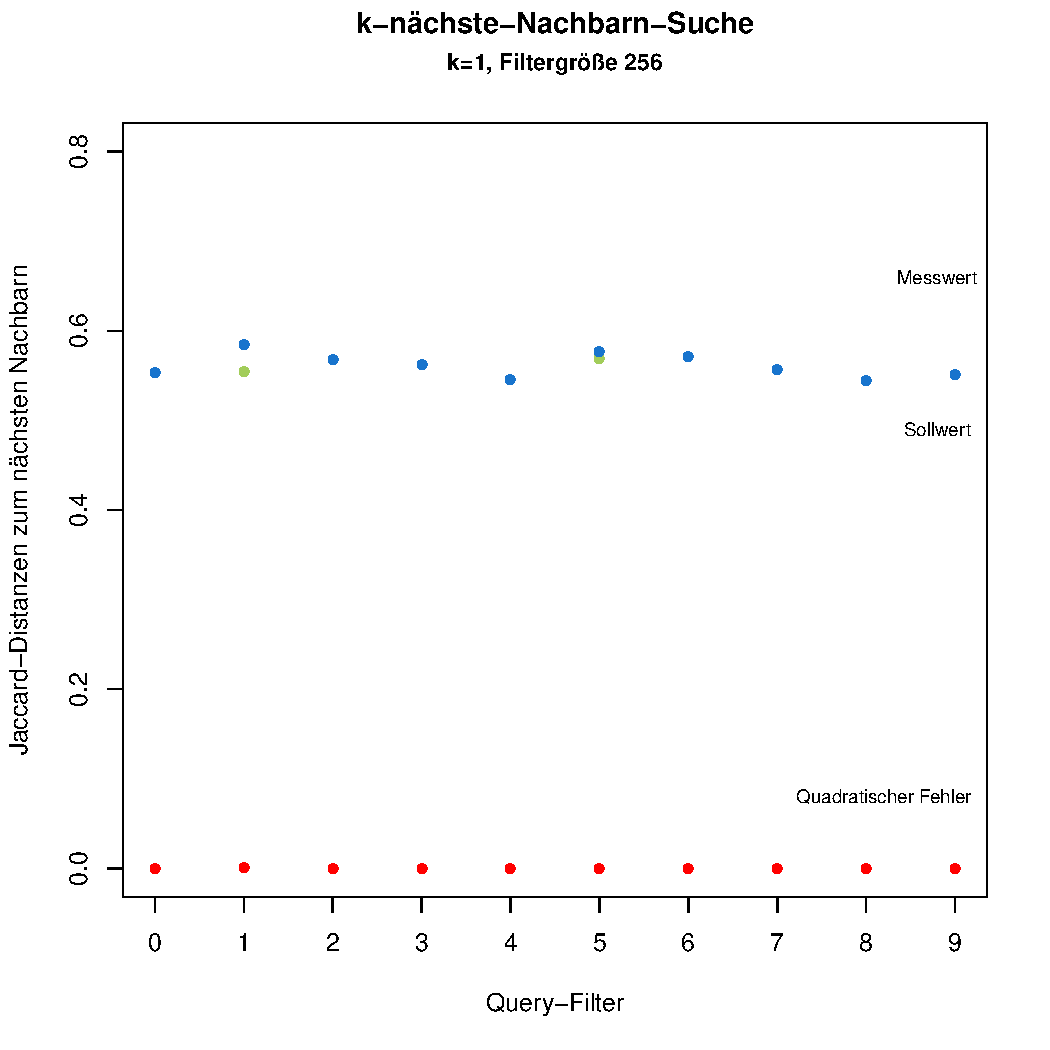
\includegraphics[scale=0.7]{pictures/nn_256.pdf}\\
  	\caption[Ergebnisqualität der nächste-Nachbarn-Suche für 256 Bit-Bloom-Filter]{Ergebnisqualität der nächste-Nachbarn-Suche für 256 Bit-Bloom-Filter.}\label{fig:pic7}
 	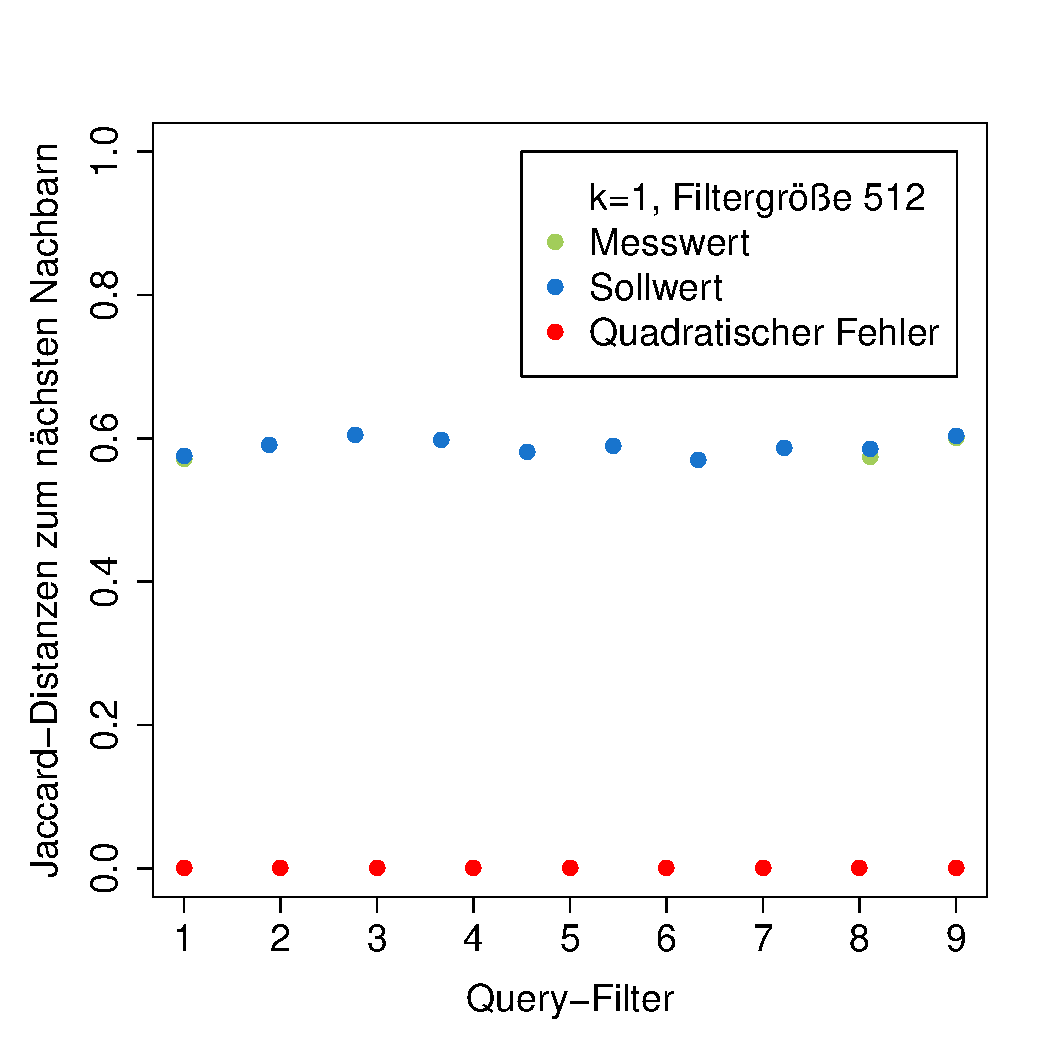
\includegraphics[scale=0.7]{pictures/nn_512.pdf}\\
  	\caption[Ergebnisqualität der nächste-Nachbarn-Suche für 256 Bit-Bloom-Filter]{Ergebnisqualität der nächste-Nachbarn-Suche für 512 Bit-Bloom-Filter.}\label{fig:pic8}
\end{figure}
Abbildungen \ref{fig:pic9} -- \ref{fig:pic12} stellen die Ergebnisqualität der 3-nächste-Nachbarn-Suche dar. Die Sollwerte sind darin in drei Grünstufen markiert, die Messwerte sind in drei Blaustufen markiert. Der mittlere quadratische Fehler der Messwerte gegenüber den Sollwerten ist in Rot angegeben.
\begin{figure}
	\centering
	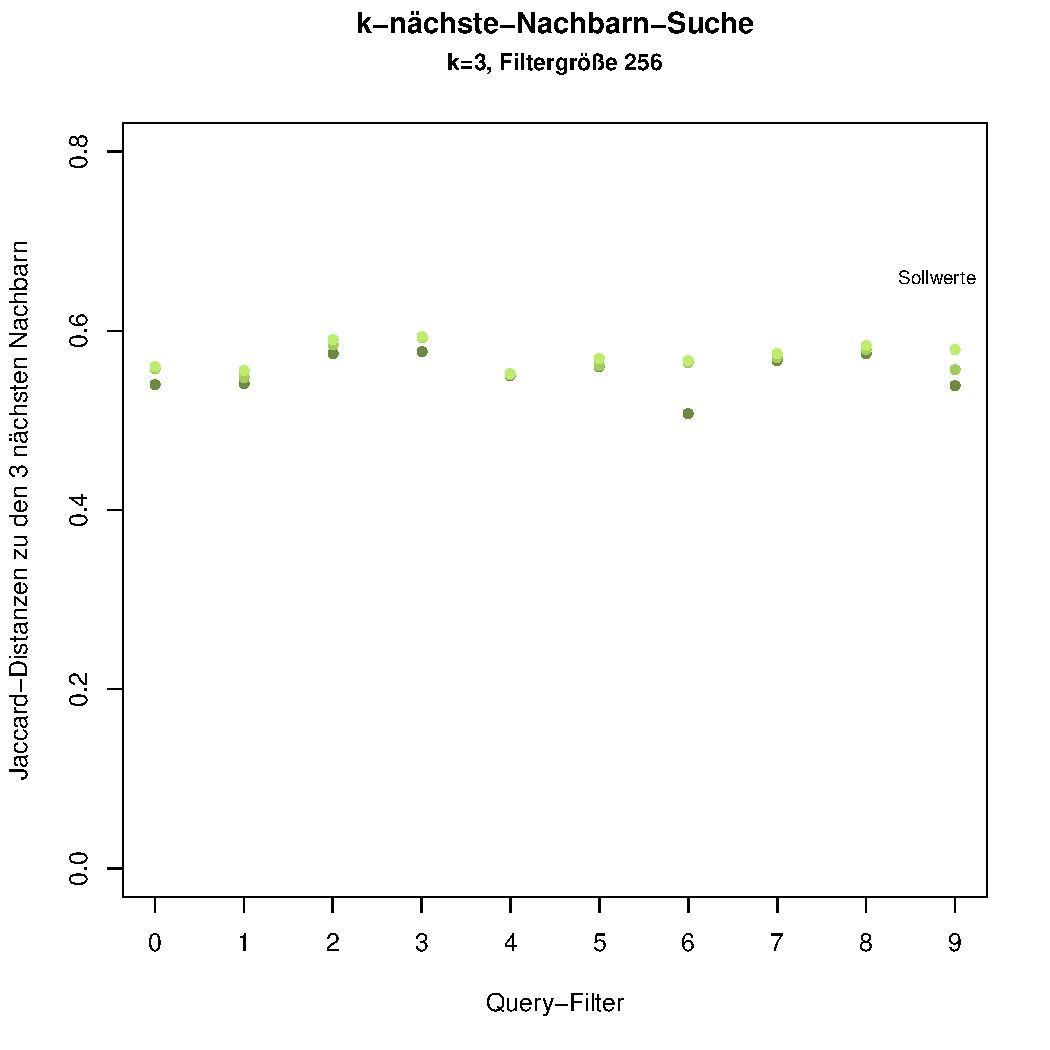
\includegraphics[scale=0.7]{pictures/nn3_256-1.pdf}\\
	\caption[Sollwerte der 3-nächste-Nachbarn-Suche für 256 Bit-Bloom-Filter]{Sollwerte der 3-nächste-Nachbarn-Suche für 256 Bit-Bloom-Filter.}\label{fig:pic9}
	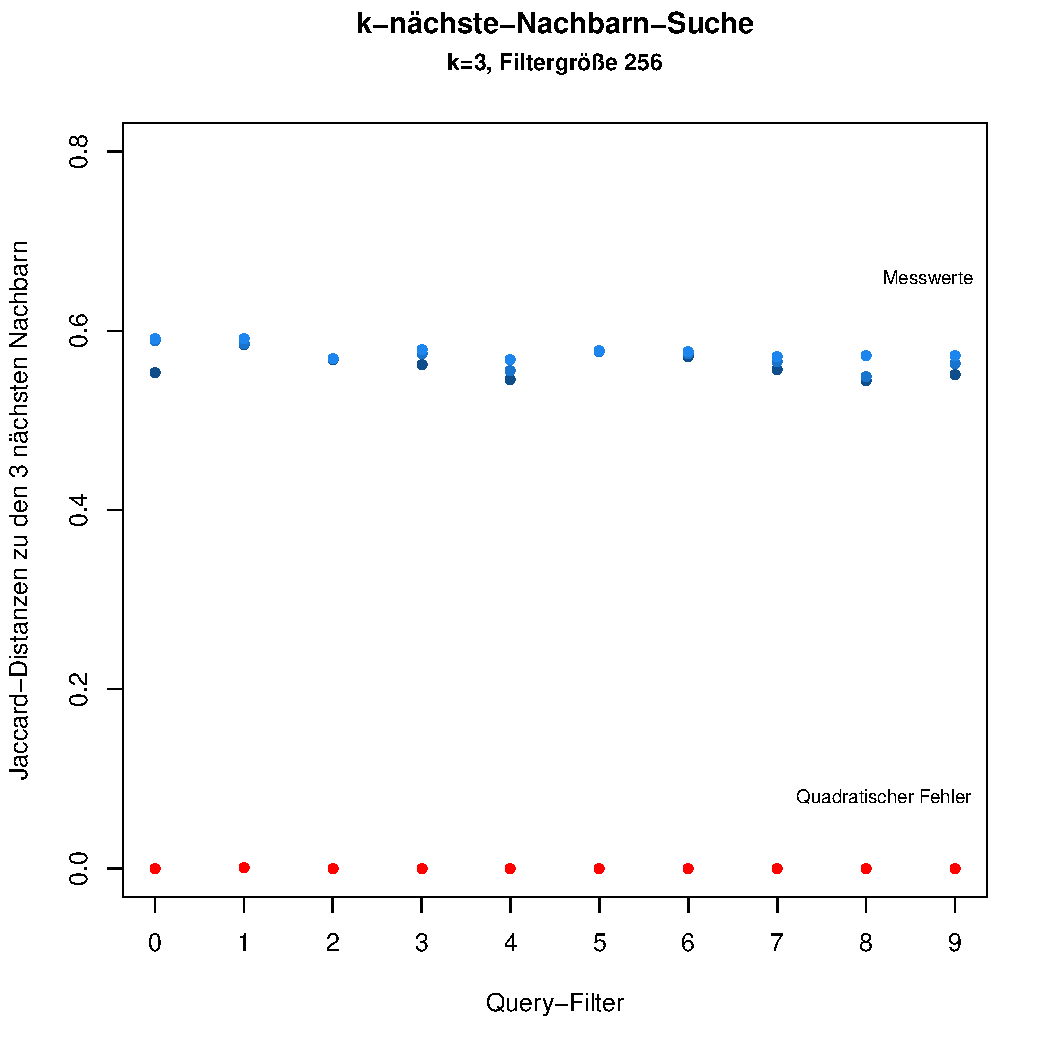
\includegraphics[scale=0.7]{pictures/nn3_256-2.pdf}\\
	\caption[Messwerte der 3-nächste-Nachbarn-Suche für 512 Bit-Bloom-Filter]{Messwerte der 3-nächste-Nachbarn-Suche für 512 Bit-Bloom-Filter.}\label{fig:pic10}
\end{figure}
\begin{figure}[hptb]
	\centering
	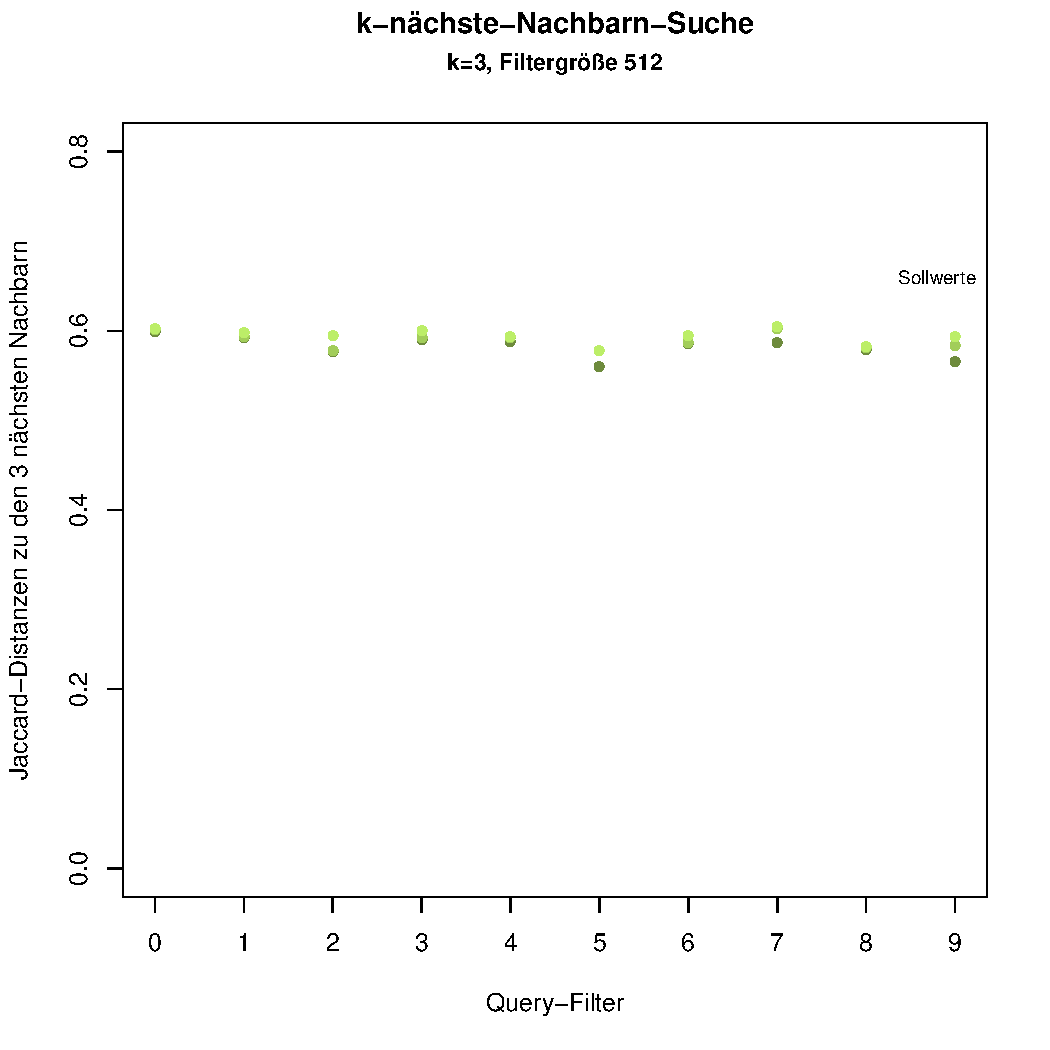
\includegraphics[scale=0.7]{pictures/nn3_512-1.pdf}\\
	\caption[Sollwerte der 3-nächste-Nachbarn-Suche für 512 Bit-Bloom-Filter]{Sollwerte der 3-nächste-Nachbarn-Suche für 512 Bit-Bloom-Filter.}\label{fig:pic11}
	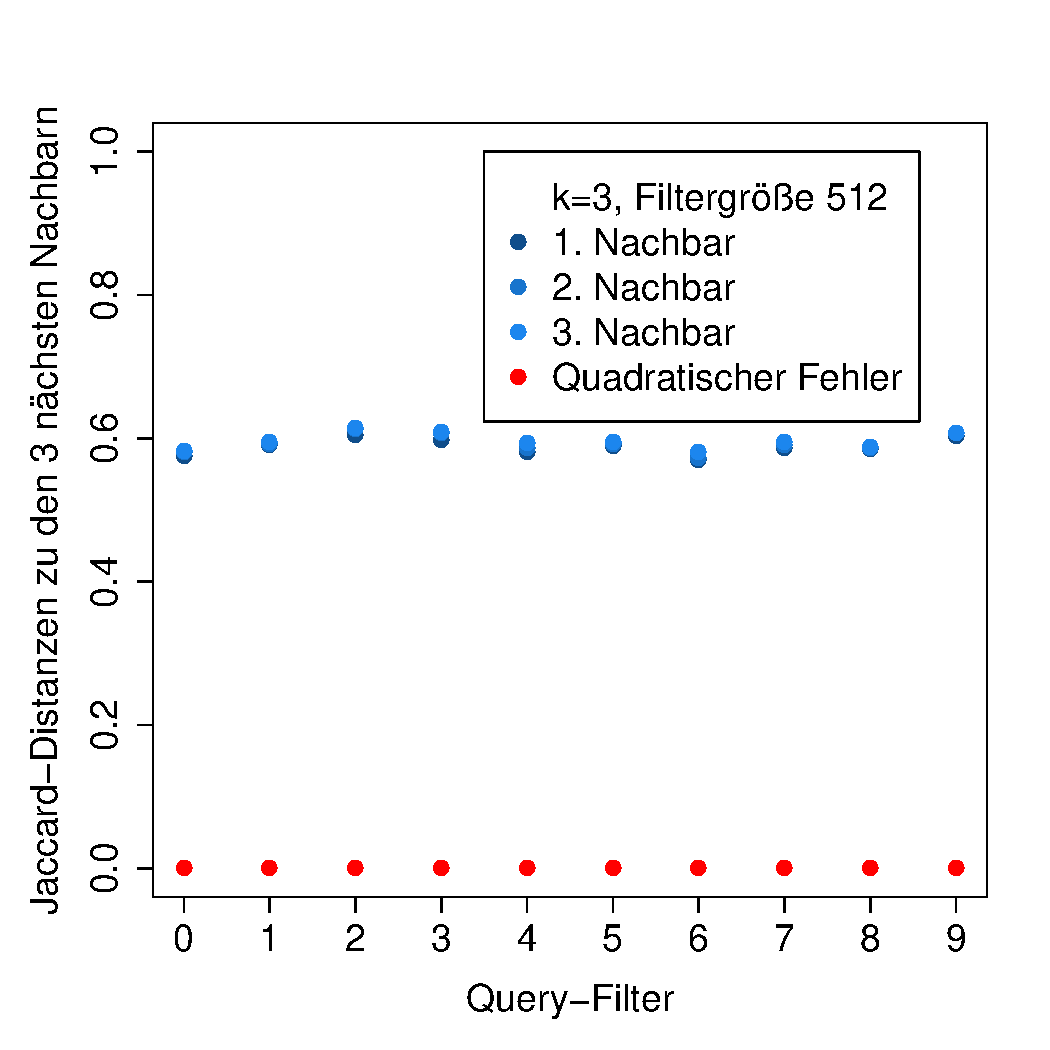
\includegraphics[scale=0.7]{pictures/nn3_512-2.pdf}\\
	\caption[Messwerte der 3-nächste-Nachbarn-Suche für 512 Bit-Bloom-Filter]{Messwerte der 3-nächste-Nachbarn-Suche für 512 Bit-Bloom-Filter.}\label{fig:pic12}
\end{figure}
\paragraph*{CPU-Zeit}
Abbildungen \ref{fig:pic13} und \ref{fig:pic14} stellen die CPU-Zeit zur Ausführung der nächste-Nachbarn-Suche dar. Die Ergebnisse für den BloomFilterTree sind darin blau, die Ergebnisse für die unsortierte Liste grün markiert.  
\begin{figure}[hptb]
	\centering
	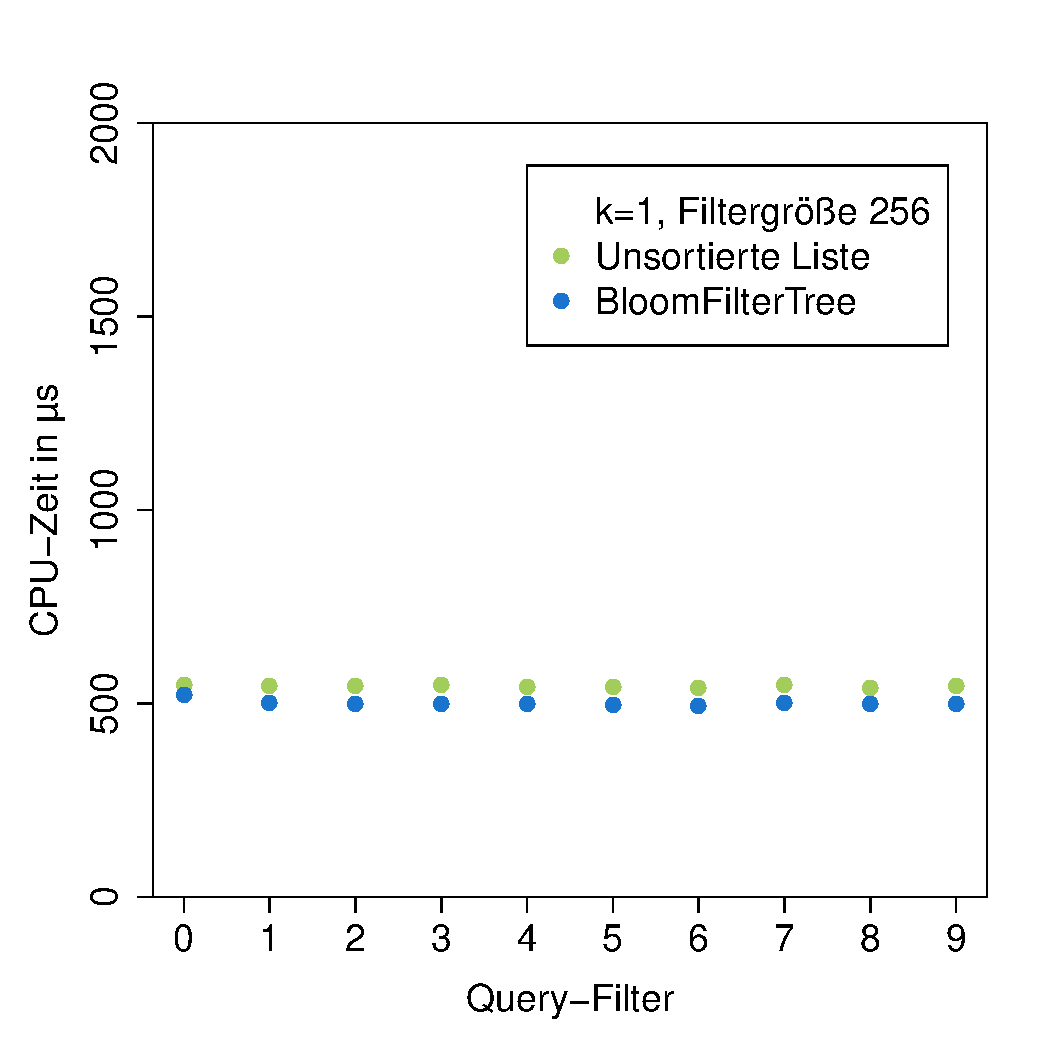
\includegraphics[scale=0.7]{pictures/cputime_nn_256.pdf}\\
	\caption[CPU-Zeit für nächste-Nachbarn-Suche mit 256 Bit-Bloom-Filtern]{CPU-Zeit für \textit{k}-nächste-Nachbarn-Suche mit 256 Bit-Bloom-Filtern.}\label{fig:pic13}
	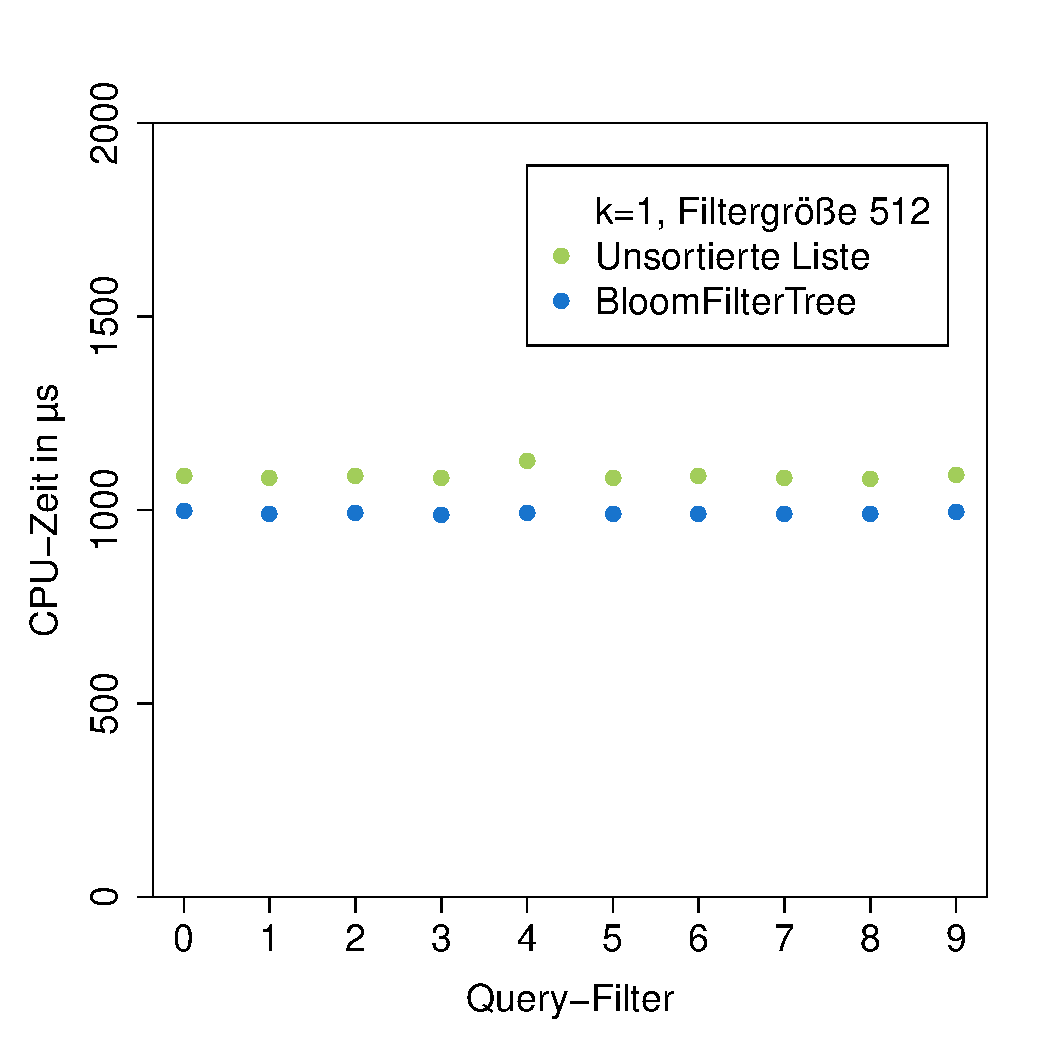
\includegraphics[scale=0.7]{pictures/cputime_nn_512.pdf}\\
	\caption[CPU-Zeit für nächste-Nachbarn-Suche mit 512 Bit-Bloom-Filtern]{CPU-Zeit für \textit{k}-nächste-Nachbarn-Suche mit 512 Bit-Bloom-Filtern.}\label{fig:pic14}
\end{figure}
Abbildungen \ref{fig:pic15} und \ref{fig:pic16} stellen die CPU-Zeit zur Ausführung der 3-nächste-Nachbarn-Suche dar. Die Ergebnisse für den BloomFilterTree sind darin blau, die Ergebnisse für die unsortierte Liste grün markiert.  
\begin{figure}[hptb]
	\centering
	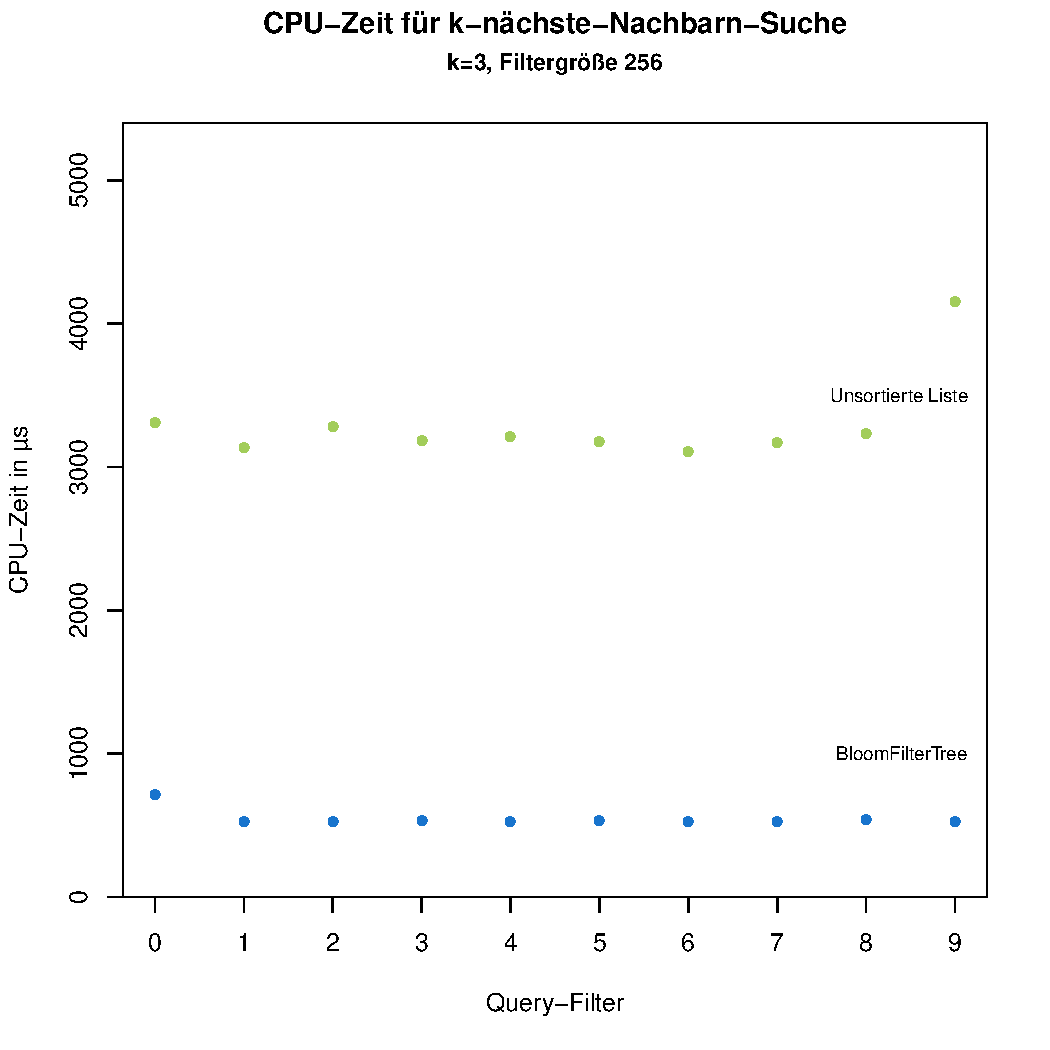
\includegraphics[scale=0.7]{pictures/cputime_nn3_256.pdf}\\
	\caption[CPU-Zeit für 3-nächste-Nachbarn-Suche mit 256 Bit-Bloom-Filtern]{CPU-Zeit für nächste-Nachbarn-Suche mit 256 Bit-Bloom-Filtern.}\label{fig:pic15}
	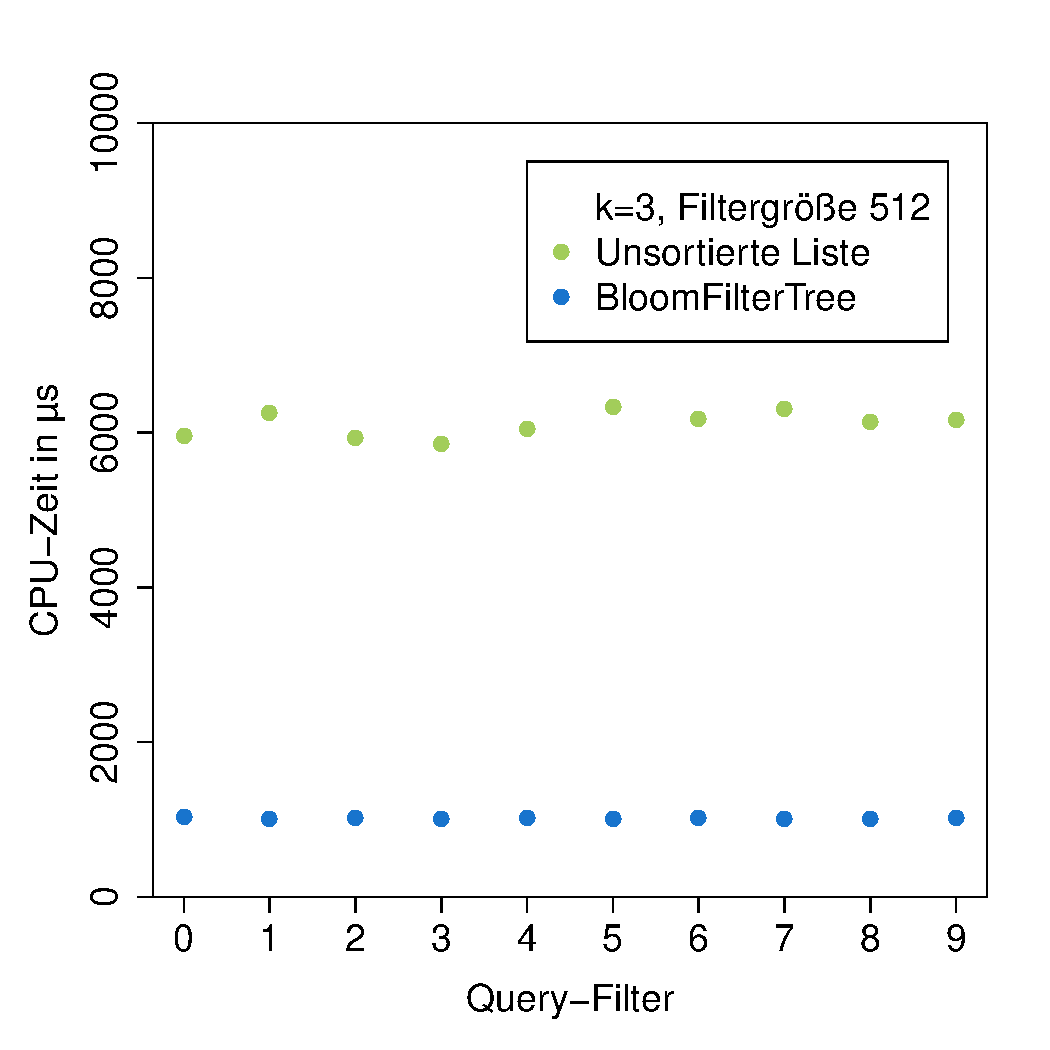
\includegraphics[scale=0.7]{pictures/cputime_nn3_512.pdf}\\
	\caption[CPU-Zeit für 3-nächste-Nachbarn-Suche mit 512 Bit-Bloom-Filtern]{CPU-Zeit für nächste-Nachbarn-Suche mit 512 Bit-Bloom-Filtern.}\label{fig:pic16}
\end{figure}
\paragraph*{Speicherbedarf}
Abbildung \ref{fig:pic17} stellt den Speicherbedarf der angelegten Objekte dar. Der Speicherbedarf für Objekte vom Typ BloomFilterTree ist darin blau markiert. Der Speicherbedarf für Objekte vom Typ \texttt{std::vector<BloomFilter>} ist grün markiert. 
\begin{figure}[hptb]
	\centering
	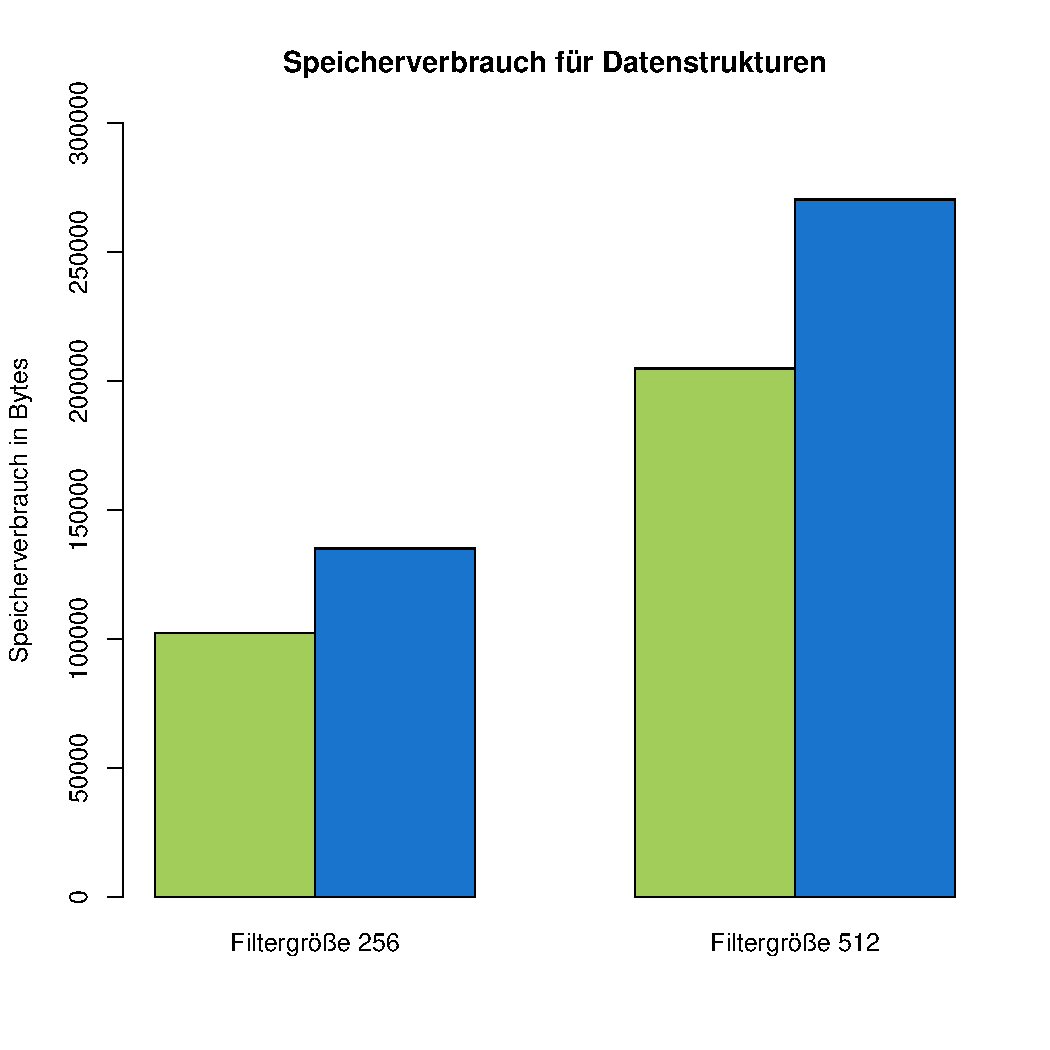
\includegraphics[scale=0.7]{pictures/mem.pdf}\\
	\caption[Speicherbedarf für BloomFilterTree und unsortierte Liste]{Speicherbedarf für BloomFilterTree und unsortierte Liste.}\label{fig:pic17} 
\end{figure}	
\paragraph*{Komplexität}
Abbildung \ref{fig:pic18} stellt die Komplexität der k-nächste-Nachbarn-Suche wie in Abschnitt \ref{sec:versuchsaufbau} beschrieben als Anzahl der zur Anfragebearbeitung nötigen Vergleiche dar. Die Ergebnisse für den BloomFilterTree sind darin blau, die Ergebnisse für die unsortierte Liste grün markiert.
\begin{figure}[hptb]
	\centering
	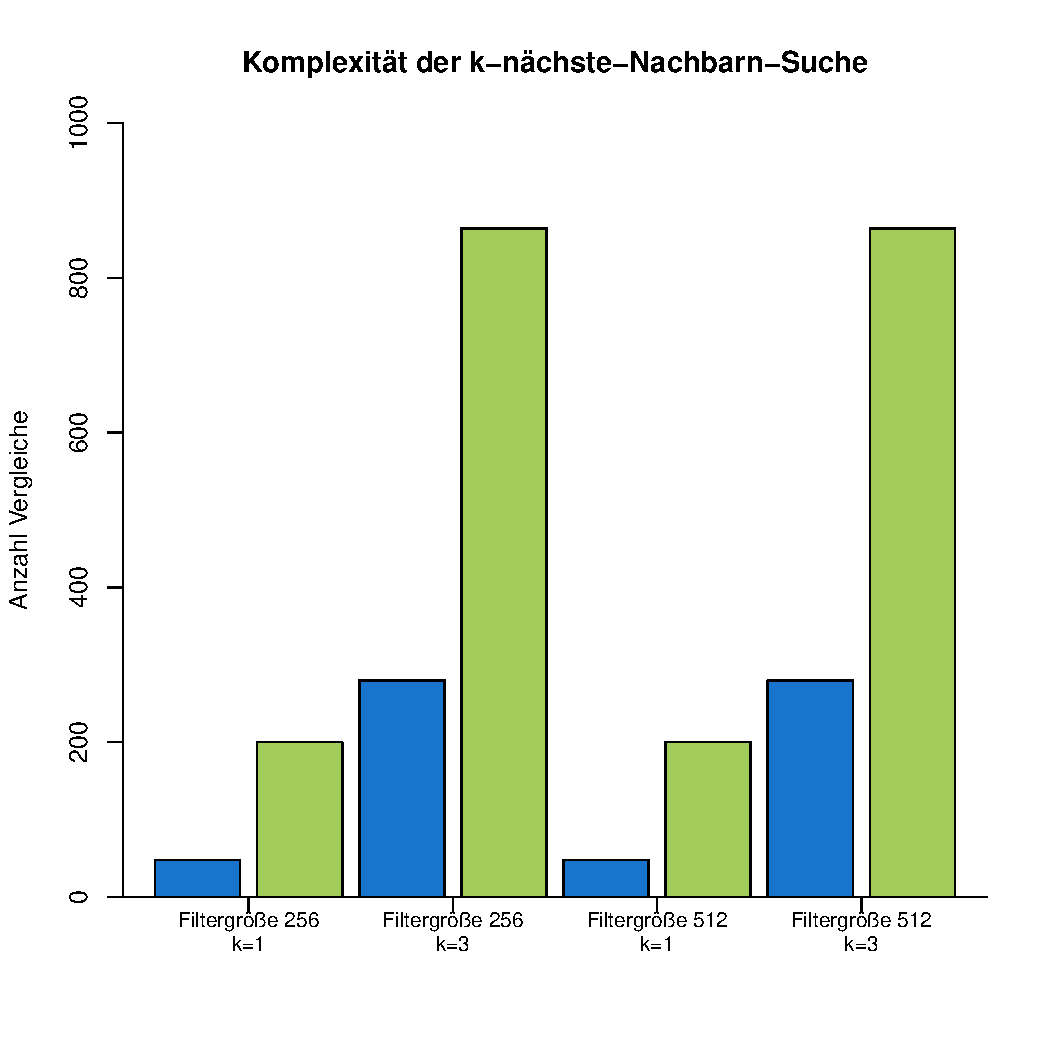
\includegraphics[scale=0.7]{pictures/compl.pdf}\\
	\caption[Anzahl zur \textit{k}-nächste-Nachbarn-Suche benötigter Vergleiche]{Anzahl zur \textit{k}-nächste-Nachbarn-Suche benötigter Vergleiche.}\label{fig:pic18}
\end{figure} 
\paragraph*{Aufbaukosten}
Abbildung \ref{fig:pic19} stellt die Aufbaukosten der angelegten Objekte dar. Die Aufbaukosten für Objekte vom Typ BloomFilterTree sind darin blau markiert. Die Aufbaukosten für Objekte vom Typ \texttt{std::vector<BloomFilter>} sind grün markiert. 
\begin{figure}[hptb]
	\centering
	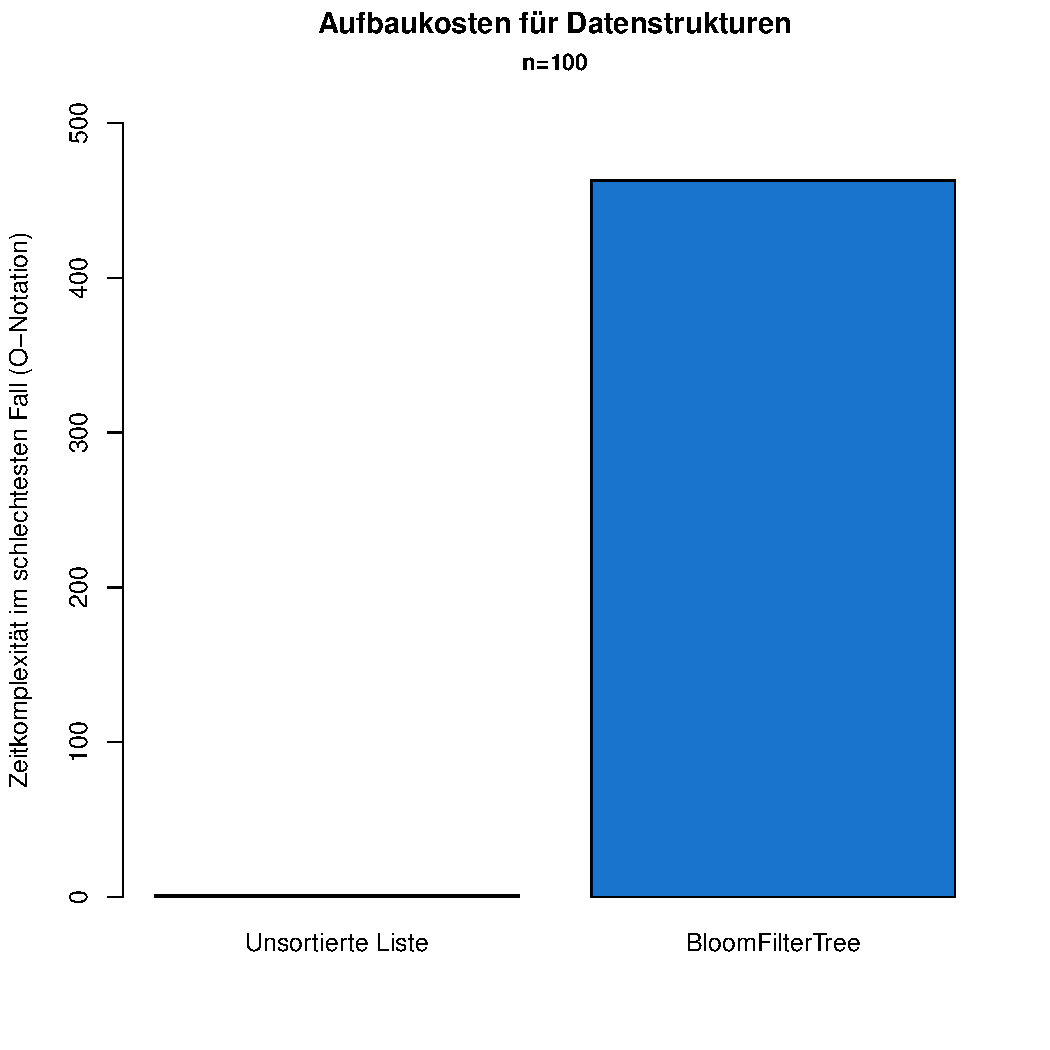
\includegraphics[scale=0.7]{pictures/cost.pdf}\\
	\caption[Aufbaukosten für BloomFilterTree und unsortierte Liste]{Aufbaukosten für BloomFilterTree und unsortierte Liste.}\label{fig:pic19}
\end{figure}
\newpage
\section{Interpretation}\label{sec:interpretation}
Wie in Abschnitt \ref{sec:datensatz} dargestellt, wurde die Evaluation mit zehn Anfragefiltern pro Experiment durchgeführt. Die soeben präsentierten Ergebnisse sind also dazu geeignet, den Mittelwert über einem Anfragevektor zu bilden und etwaige Ausreißer zu erkennen. Das gilt insbesondere für die Ergebnisse der CPU-Zeitmessung, die in der Regel wegen schwankender Nutzlast der verwendeten Maschine und nicht exakt vorhersehbaren CPU-Schedulings gewissen Schwankungen unterliegen. Demnach kann hierfür das Minimum der erzielten Werte als Benchmark für die \textit{k}-nächste-Nachbarn-Suche angesehen werden. 
\paragraph*{Ergebnisqualität}
Die Ergebnisse der \textit{k}-nächste-Nachbarn-Suche stimmen zum größten Teil mit den Sollwerten überein. Bei der nächsten-Nachbarn-Suche mit 256 Bit-Bloom-Filtern treten zwei abweichende Ergebnisse auf (vgl. Abbildung \ref{fig:pic7}). Bei der 3-nächste-Nachbarn-Suche mit 256-Bit-Filtern treten bei 30 Ergebnissen fünf abweichende Einzelergebnisse auf. Bei der 3-nächste-Nachbarn-Suche mit 512-Bit-Filtern treten bei 30 Ergebnissen sechs abweichende Einzelergebnisse auf. 

Der quadratische Fehler für diese Fälle beträgt bei der nächste-Nachbarn-Suche mit 256 Bit-Bloom-Filtern maximal 0.0008548022, andernfalls 0. Bei der 3-nächste-Nachbarn-Suche mit 256 Bit-Bloom-Filtern beträgt der mittlere quadratische Fehler bei abweichenden Messwerten maximal 0.0002956207, andernfalls 0. Bei der 3-nächste-Nachbarn-Suche mit 512 Bit-Bloom-Filtern beträgt er maximal 0.00008640455, andernfalls 0.

Das bedeutet: Nächste-Nachbarn-Anfragen werden mit dem entwickelten Verfahren in den meisten Fällen korrekt beantwortet. Mit einigen wenigen Fällen werden suboptimale Antworten zurückgegeben. Diese sind dennoch als "`gute"' Antworten bezüglich des verwendeten Distanzmaßes und des maximalen quadratischen Fehlers zu bezeichnen. Dieses Resultat ist essentiell für die Bewertung des entwickelten Verfahrens. Es kann nur dann zuverlässig eingesetzt werden, wenn es in einem Großteil der Fälle zufriedenstellende Ergebnisse bzw. optimale Antworten liefert. 
\paragraph*{CPU-Zeit}
Die drastisch reduzierte CPU-Zeit ist als entscheidender Vorteil des entwickelten Verfahrens zu betrachten. In der verwendeten Versuchsanordnung kommt sie vor allem bei der 3-nächste-Nachbarn-Suche zum Tragen. Abbildung \ref{fig:multipic1} stellt die jeweils erreichte CPU-Zeitersparnis gegenüber:
\begin{figure}[hpbt]
 \centering
  %%----start of first subfigure----
  \subfloat[CPU-Zeitersparnis für nächste-Nachbarn-Suche mit 256-Bit-Bloom-Filtern]{
   \label{fig:multipic1:a} %% label for first subfigure
   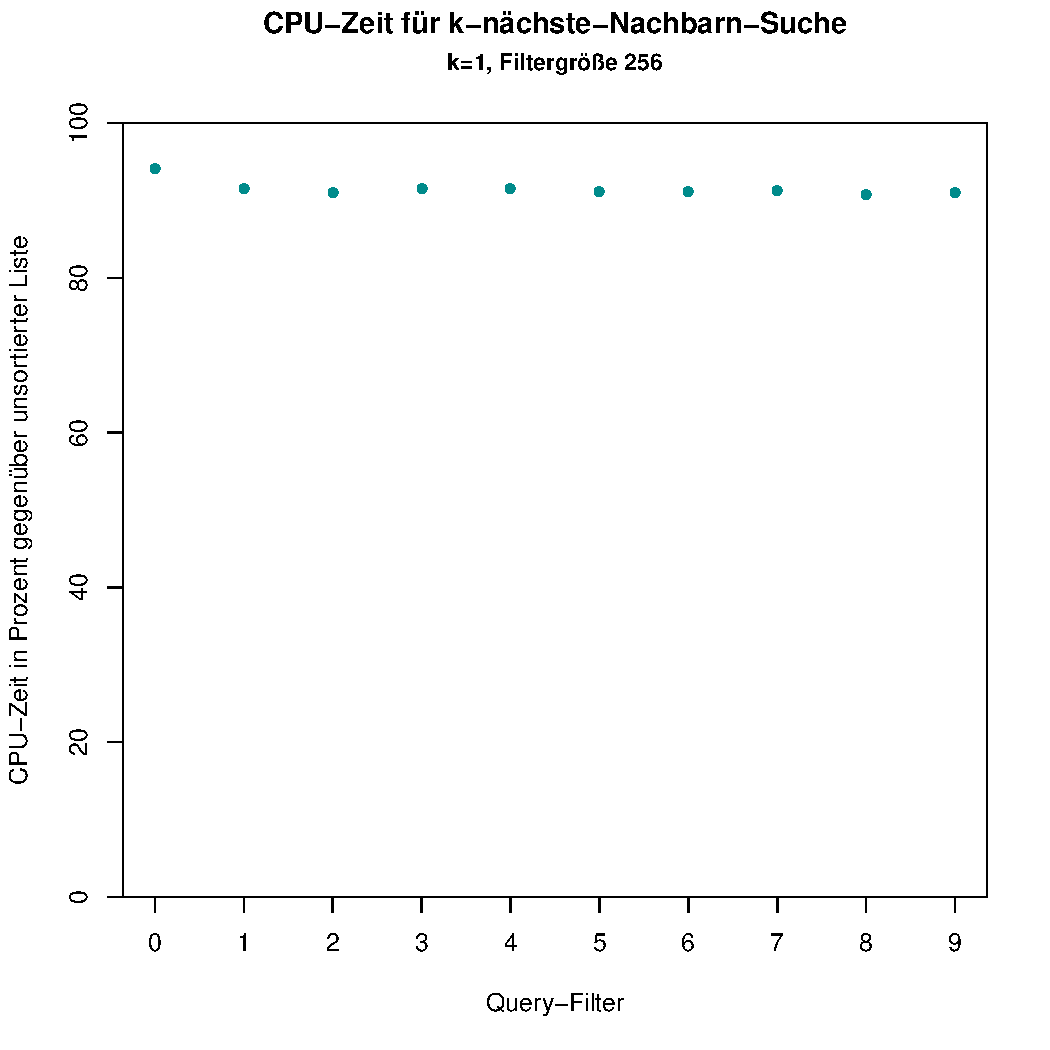
\includegraphics[width=0.48\linewidth]{pictures/percent_time_nn_256.pdf}}
  \hspace{0.01\textwidth}
  %%----start of second subfigure----
  \subfloat[CPU-Zeitersparnis für nächste-Nachbarn-Suche mit 512-Bit-Bloom-Filtern]{
   \label{fig:multipic1:b} %% label for second subfigure
   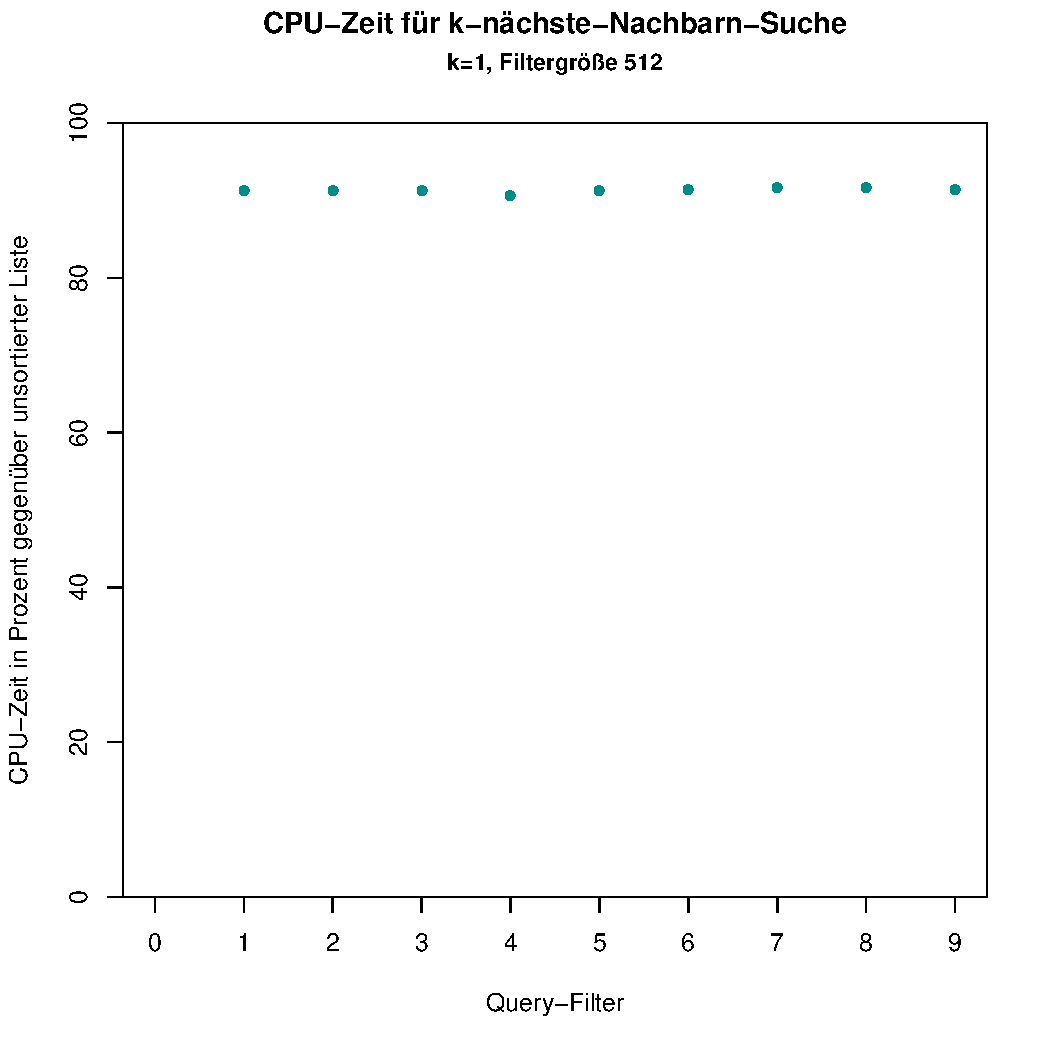
\includegraphics[width=0.48\linewidth]{percent_time_nn_512.pdf}}\\[0pt] % horizontal break
  %%----start of third subfigure----
  \subfloat[CPU-Zeitersparnis für 3-nächste-Nachbarn-Suche mit 256-Bit-Bloom-Filtern]{
   \label{fig:multipic1:c} %% label for third subfigure
   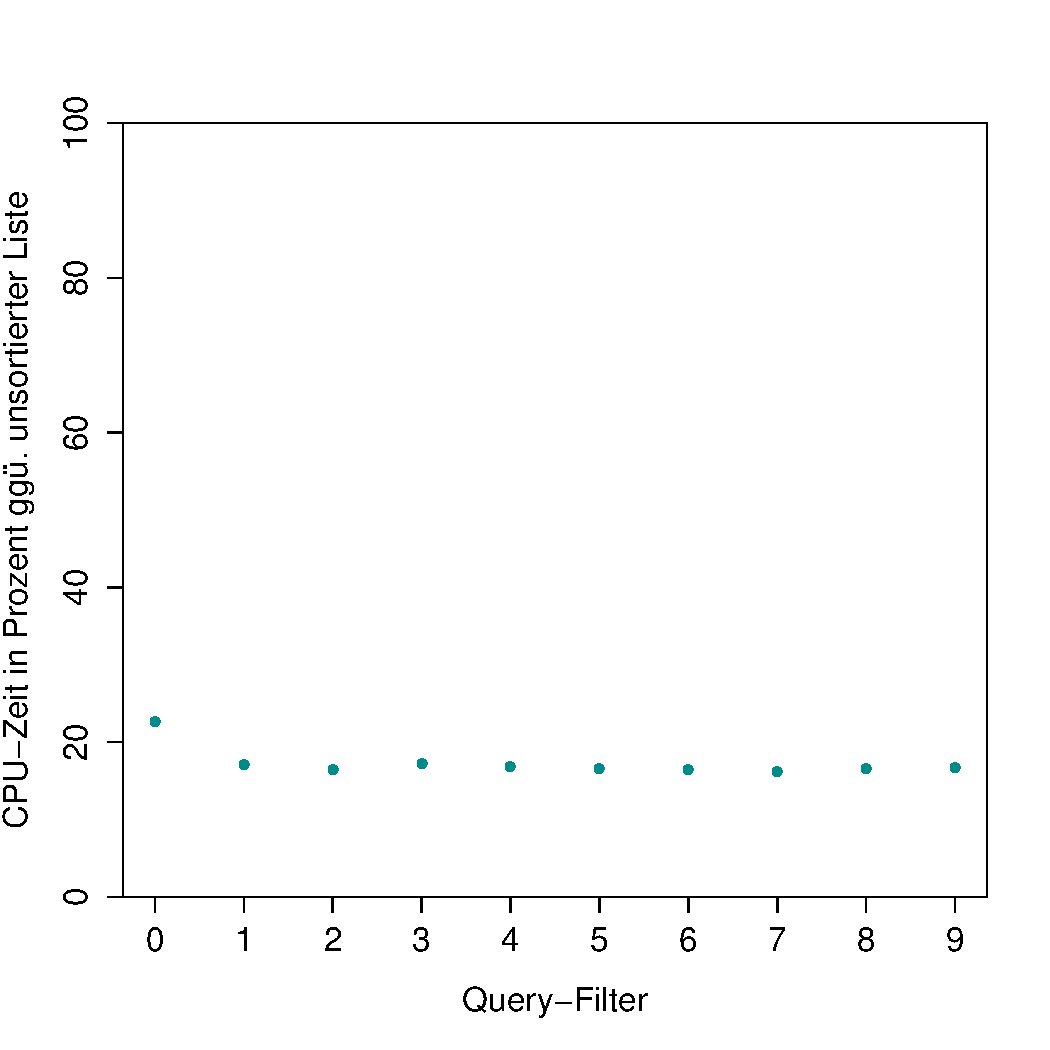
\includegraphics[width=0.48\linewidth]{pictures/percent_time_nn3_256.pdf}}
  \hspace{0.01\textwidth}
  %%----start of fourth subfigure----
  \subfloat[CPU-Zeitersparnis für 3-nächste-Nachbarn-Suche mit 512-Bit-Bloom-Filtern]{
   \label{fig:multipic1:d} %% label for fourth subfigure
   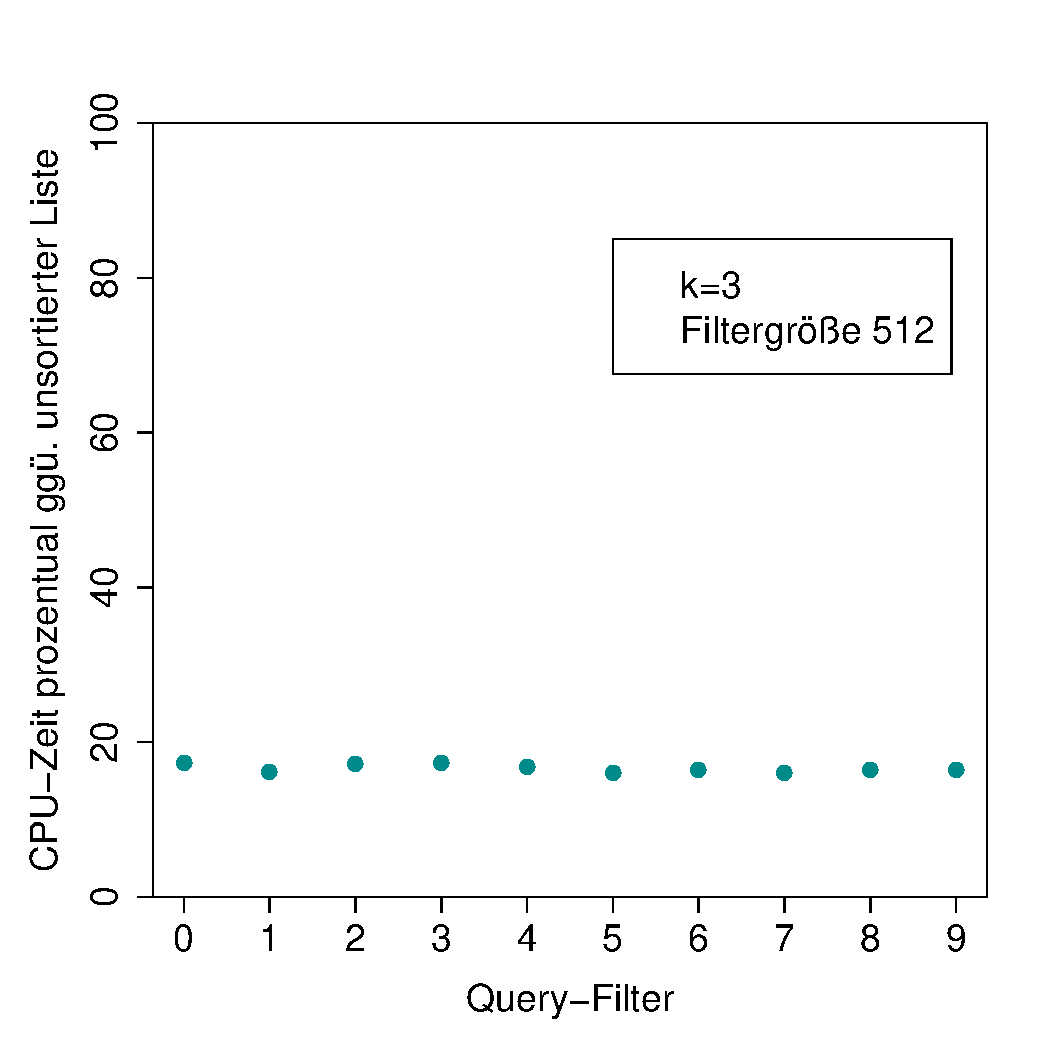
\includegraphics[width=0.48\linewidth]{pictures/percent_time_nn3_512.pdf}}
 \caption[CPU-Zeitersparnis für k-nächste-Nachbarn-Suche im BloomFilterTree]{CPU-Zeitersparnis für k-nächste-Nachbarn-Suche im BloomFilterTree.}
 \label{fig:multipic1} %% label for entire figure
\end{figure}
Daran wird deutlich: Die Zeitersparnis wächst mit dem Parameter \textit{k} und der Filtergröße, doch auch bei $k=1$ wird bereits CPU-Zeit eingespart. Es ist zu erwarten, dass bei größeren BloomFilterTree-Objekten, höheren Anzahlen an Filtern und ggf. größeren Filtern die Zeitersparnis noch deutlich gesteigert werden kann: 

Beim hier verwendeten Versuchsaufbau werden i.d.R Bäume mit drei Ebenen aufgebaut, d.h. bei einer Punktanfrage wird auch bei bestehenden Teil- und Obermengenbeziehungen ein großer Teilbaum durchsucht bzw. ein großer Bereich der Blattebene traversiert. Bei größerer Höhe des Baums durch mehr eingefügte Filter kommen damit die Vorteile des entwickelten Verfahrens deutlicher zum Tragen. Wie in Abbildung \ref{fig:multipic1} erkennbar, gilt ebenso für höhrere Filtergrößen. Die CPU-Zeitersparnis zeigt sich bei Anfragen mit $k>1$ besonders deutlich. Auch hier ist zu erwarten, dass sich die Vorteile des entwickelten Verfahrens bei höheren Bäumen und Filteranzahlen sowie größeren Filtern noch deutlich stärker zeigen.

Wie in Abschnitt \ref{sec:b+bäume} dargestellt, ist die Komplexität der Suchoperation im B$^+$-Baum abhängig vom Parameter \textit{t} ab, d.h. dem Grad des Baumes. Die hier verwendeten BloomFilterTree-Objekte haben Grad 3, d.h. der maximale Fan-out beträgt 7. Dieser Parameter kann beim Anlegen eines BloomFilterTree-Objekts in der eigenen Implementierung frei gewählt werden. In der Praxis werden deutlich höhere Verzweigungsgrade verwendet, z.B. mit 10.000 Elemente pro innerem Knoten beim Einsatz in Datenbank-Management-Systemen. Es ist daher anzunehmen, dass die Anwendung für ein Szenario mit deutlich höheren Parameterwerten gut geeignet wäre. 
\paragraph*{Speicherbedarf}
Der zusätzliche Speicherbedarf beim BloomFilterTree gegenüber einem Bloom-Filter-Vektor ergibt sich durch die Allokierung eines Vereinigungsfilters für jeden Knoten. Er ist somit abhängig von der Anzahl der Knoten im Baum. Mit dem verwendeten Versuchsaufbau liegt er um 32\% für den BloomFilter gegenüber einem Bloom-Filter-Vektor. Auch hier ließe sich durch eine geringere Knotenanzahl, d.h. BloomFilterTree-Objekte mit höherem Verzweigungsgrad, noch Speicherplatz einsparen. 
\paragraph*{Komplexität}
Auch bezüglich der Zeitkomplexität, d.h. der Abschätzung der notwendigen Berechnungsschritte unabhängig von der gewählten Plattform, zeigt das entwickelte Verfahren erfreuliche Ergebnisse. Die Anzahl der nötigen Vergleiche bei der \textit{k}-nächste-Nachbarn-Suche beträgt 24\% bzw. 32\% beim BloomFilterTree gegenüber der unsortierten Liste. Auch hier ist zu erwarten, dass sich die Ergebnisse bei höheren Bäumen noch verbessern lassen, da bei der \textit{k}-nächste-Nachbarn-Suche nur der beste Pfad verfolgt wird. Bei höheren Bäumen werden somit mehr bzw. größere Teilbäume abgeschnitten und müssen nicht betrachtet werden. 
\paragraph*{Aufbaukosten}
Die Kosten für den Aufbau der Indexstruktur sind erwartungsgemäß ein Wermutstropfen. Auch wenn in der Praxis niedrigere Werte zu erwarten sind, da weniger als \textit{n} freie und "`gute"' IDs sortiert werden müssen, liegen die Aufbaukosten in $O(n\ast log(n))$. Das ist offensichtlich ein starker Zuwachs gegenüber einer unsortierten Liste, die sich z.B. durch ein Objekt vom Typ \texttt{std::vector} realisieren lässt. Andererseits kann davon ausgegangen werden, dass die Aufbaukosten in AMBIENCE deutlich seltener anfallen als z.B. in einem Verteilten System mit häufigem Ausscheiden und Hinzukommen von Knoten wie in den Abschnitten \ref{sec:bloom-netzwerk} und \ref{sec:bloom-index} beschrieben.
    \chapter{Conclusions}\label{conclusions}
%
% =================================================================================================
% place your appendix here
% -------------------------------------------------------------------------------------------------
%
    \appendix
    % % -------------------------------------------------------------------------------------------------
%      MDSG Latex Framework
%      ============================================================================================
%      File:                  appendix.tex
%      Author(s):             Michael Duerr
%      Version:               1
%      Creation Date:         30. Mai 2010
%      Creation Date:         30. Mai 2010
%
%      Notes:                 - Place your appendix here
%                             - Use the same commands (`chapter', `section', ...) as in main text
% -------------------------------------------------------------------------------------------------
%
\chapter{Anhang}\label{ch:anhang}
\section{Die Klasse \texttt{BloomFilterTree}}\label{sec:BloomFilterTree.hpp}
\small{
\begin{verbatim}
//  BloomFilterTree.hpp, Judith Greif
//  Description: Header for class BloomFilterTree

#ifndef BloomFilterTree_hpp
#define BloomFilterTree_hpp

#include "BloomFilterNode.hpp"
#include "BloomFilterIndexNode.hpp"
#include "BloomFilterLeaf.hpp"

using namespace std;

class BloomFilterTree {
    
private:
    int t;                          // Order = minimum degree
    int filtersize;                 // Size of associated Bloom filters (# of bits)
    
public:
    BloomFilterNode *root;          // Pointer to root node   
    BloomFilterTree(int _t, int _s);
    ~BloomFilterTree();   
    BloomFilterNode *getRoot();
    
    // Tree management
    void traverse();
    void traverseFilters();
    double computeMinJaccard(BloomFilter *filter);
    double computeMaxJaccard(BloomFilter *filter);
    int getMinJaccardKey(BloomFilter *filter);
    BloomFilter *getMinJaccardFilter(BloomFilter *filter);
    int getMinKey();
    int getMaxKey();
    vector<BloomFilter> collectAllFilters();
    int countFilters();
    int countUnionFilters(); 
    int computeSubsetId(BloomFilter *filter);
    int computeSupersetId(BloomFilter *filter);
    bool contains(int k);
    BloomFilterNode *search(int k);
    vector<pair<int, double>>computeAllDistances(BloomFilter *filter);
    vector<pair<int, double>>computekDistances(BloomFilter *filter, int k);
    int countLeaves(); 
    
    // Measurement and comparison
    vector<pair<BloomFilter, double>> compare(BloomFilter *filter, int k);
    vector<int> compareMem();
    vector<double> compareConstrCost();
    vector<int> compareComplSimQuery(BloomFilter *filter);
    vector<int> compareComplSimQueryVec(BloomFilter *filter, int k);
    
    // Insertion
    void insert(BloomFilter *filter);
    void insertAsSets(BloomFilter *filter);
    
    // Similarity queries
    BloomFilter *simQuery(BloomFilter *filter);
    vector<BloomFilter*> simQueryVec(BloomFilter *filter, int k);
};

#endif
\end{verbatim}
}
\newpage
\section{Die Klasse \texttt{BloomFilter}}\label{sec:BloomFilter.hpp}
\small{
\begin{verbatim}
//  BloomFilter.hpp, Judith Greif
//  Description: Header for class BloomFilter

#ifndef BloomFilter_hpp
#define BloomFilter_hpp

#include <iostream>
#include <vector>
#include <cstdlib>
#include <random>
#include <math.h>
#include <string>
#include <functional>

using namespace std;

const int NUM_FILTERS = 100;
const int NUM_ELEMENTS = 50;
const int NUM_QUERYFILTERS = 10;
const int seed = rand();

class BloomFilter {
    
private:
    int id;
    int count;                  // # of elements inserted
    int size;                   // # of bits
    int d;                      // # of hash functions
    int *data;
    
public:
    BloomFilter();
    BloomFilter(const BloomFilter& fSource);
    BloomFilter(int _id, int _size);
    ~BloomFilter();   
    BloomFilter & operator = (const BloomFilter &fSource);   
    void setId(int value);
    int getId();
    int getSize();
    void setValue(int index, int value);
    int *getData();   
    void printData();
    void printArr();
    void initRandom();
    double fractionOfZeros();
    double eSize();
    BloomFilter *logicalOr(BloomFilter *filter);
    BloomFilter *logicalAnd(BloomFilter *filter);
    bool isSubset(BloomFilter *filter);
    bool isSuperset(BloomFilter *filter);
    int mySupersetCount();
    int mySubsetCount();
    int binomialCoefficient(int n, int k);
    int setOnes();
    int setZeros();
    int validOnes();
    int possibleFreeZeros();
    int possibleAddedOnes();
    double setUnion(BloomFilter *filter) const;
    double setIntersection(BloomFilter *filter) const;
    double computeAmbienceJaccard(BloomFilter *filter);
    double computeJaccard(BloomFilter *filter) const;
    double eUnion(BloomFilter *filter);
    double eIntersect(BloomFilter *filter);
    void add(string &elem);
    void increment();
    int getNumHashes();
    bool checkCorrectFillDegree();
};

#endif
\end{verbatim}
\newpage
\section{Die Methode \texttt{computeSubsetId()} der Klasse \texttt{BloomFilterLeaf()}}\label{sec:computeSubsetId()}
\small{
\begin{verbatim}
int BloomFilterLeaf::computeSubsetId(BloomFilter *filter) {
    vector<pair<int, double>> subsets;
    vector<int> freeIds;
    vector<pair<int, int>> goodIds;
    BloomFilterLeaf *tmp = this;
    double jacc;
    int minId = filters[0]->getId()-1;
    int maxId;
    int optId;
    bool no_subsets = true;
    while (tmp != NULL) {
        
        // Collect all filters that filter is subset of
        for (int i=0; i<tmp->getCount(); i++) {
            if ((tmp->filters[i])->isSubset(filter)) {
                jacc = computeJaccard(tmp->filters[i], filter);
                subsets.push_back(make_pair(tmp->filters[i]->getId(), jacc));
                no_subsets = false;
            }
        }
        maxId = tmp->filters[tmp->getCount()-1]->getId()+1;
        tmp = tmp->getNext();
    }
    
    // Sort subsets by jacc distances in ascending order
    sort(subsets.begin(), subsets.end(), [](const pair<int, double> &left, 
    const pair<int, double> &right) {
        return left.second < right.second;
    });
    
    // Collect free ids
    tmp = this;
    freeIds.push_back(minId);
    freeIds.push_back(maxId);
    while (tmp != NULL) {
        for (int i=0; i<tmp->getCount()-2; i++) {
            for (int j=tmp->filters[i]->getId()+1; j<tmp->filters[i+1]->getId(); j++) {
                if (j<tmp->filters[i+1]->getId()) {
                    freeIds.push_back(j);
                }
            }
            if (tmp->getCount() < tmp->getMax()) {
                if (tmp->getNext() != NULL) {
                    int start = tmp->filters[tmp->getCount()-1]->getId()+1;
                    int last = tmp->getNext()->filters[0]->getId();
                    for (int j=start; j<last; j++) {
                        freeIds.push_back(j);
                    }
                }
            }
            
        }
        tmp = tmp->getNext();
    }
    sort(freeIds.begin(), freeIds.end(), less<int>());
    
    // If there are no subsets, return smallest free id as pair with numerical distance 0
    if (no_subsets == false) {
        
        // Determine optimal id
        // Check subsets in ascending order
        // Get next greater and smaller id
        int distNeg = subsets[0].first - minId;
        int distPos = maxId - subsets[0].first;
        for (int i=0; i<subsets.size(); i++) {
            optId = subsets[i].first;
            int j=0;
            while (freeIds[j] < subsets[i].first) {
                if (optId-freeIds[j] < optId-minId) {
                    minId = freeIds[j];
                    distNeg = optId-minId;
                }
                j++;
            }
            
            j=freeIds.size()-1;
            while (freeIds[j] > subsets[i].first) {
                if (freeIds[j]-optId < maxId-optId) {
                    maxId = freeIds[j];
                    distPos = maxId-optId;
                }
                j--;
            }
            goodIds.push_back(make_pair(minId, distNeg));
            goodIds.push_back(make_pair(maxId, distPos));
        }
        
        // Sort next smaller and greater ids by numerical distance in ascending order
        sort(goodIds.begin(), goodIds.end(), [](const pair<int, int> &left, 
        const pair<int, int> &right) {
            return left.second < right.second;
        });
    }
    else {
        goodIds.push_back(make_pair(freeIds[0], 0));
    }
    
    // Return first element
    return goodIds[0].first;
}
\end{verbatim}
}
    % further appendix
%
% =================================================================================================
% comment \listoffigures and/or \listoftables if not wanted
% -------------------------------------------------------------------------------------------------
%
    \backmatter
    % \listoffigures                                % list of figures (uncomment if wanted)
    % \listoftables                                 % list of tables (uncomment if wanted)
    % \lstlistoflistings                            % list of listings (uncomment if wanted)
%
% =================================================================================================
% place your bibliography here
% -------------------------------------------------------------------------------------------------
%
    \begin{spacing}{0.9}                          % save some space
    	   %\nocite{*}
       %\bibliographystyle{geralpha}               % for german thesis
       \bibliographystyle{alpha}                 % for english thesis
       \bibliography{bibliography}                % the location of bib file
    \end{spacing}
\end{document}
%
% =================================================================================================
% end of document
% -------------------------------------------------------------------------------------------------
%
